\documentclass[12pt]{report}

\usepackage{hcmut-report}
\usepackage{codespace}

% Sub-preambles
% https://github.com/MartinScharrer/standalone

% Encodings
\usepackage{amsmath,amssymb,gensymb,textcomp}

% Better tables
% Wide tables go to https://tex.stackexchange.com/q/332902
\usepackage{array,multicol,multirow,siunitx,tabularx}

% Better enum
\usepackage{enumitem}

% Graphics
\usepackage{caption,float}

% Code listings
\usepackage{listings}
\usepackage[table]{xcolor}

% Code style configuration
\definecolor{codegreen}{rgb}{0,0.6,0}
\definecolor{codegray}{rgb}{0.5,0.5,0.5}
\definecolor{codepurple}{rgb}{0.58,0,0.82}
\definecolor{backcolour}{rgb}{0.97,0.97,0.97}

\lstdefinestyle{mystyle}{
    backgroundcolor=\color{backcolour},   
    commentstyle=\color{codegreen},
    keywordstyle=\color{blue},
    numberstyle=\tiny\color{codegray},
    stringstyle=\color{codepurple},
    basicstyle=\ttfamily\footnotesize,
    breakatwhitespace=false,         
    breaklines=true,                 
    captionpos=b,                    
    keepspaces=true,                 
    numbers=left,                    
    numbersep=5pt,                  
    showspaces=false,                
    showstringspaces=false,
    showtabs=false,                  
    tabsize=4,
    frame=single,
    framesep=3pt,
    xleftmargin=15pt,
    framexleftmargin=15pt
}
\lstset{style=mystyle}

% TikZ for diagrams
\usepackage{tikz}
\usetikzlibrary{shapes,arrows,positioning}
\usepackage{pgfplots}
\pgfplotsset{compat=1.18}

% Allow setting >max< width of figure
% Remove if unneeded
\usepackage[export]{adjustbox} % 'export' allows adjustbox keys in \includegraphics
\usepackage{mwe}

% Chapter and section formatting
\usepackage{titlesec}
\titleformat{\chapter}[display]
  {\normalfont\huge\bfseries}{\chaptertitlename\ \thechapter}{20pt}{\Huge}
\titlespacing*{\chapter}{0pt}{-20pt}{40pt}

% Custom commands
% Remove if unneeded
\newcommand*\mean[1]{\bar{#1}}

\ocoursename{Internet of Things Application Development}
\oreporttype{Assignment Report}
\title{Smart Environmental Monitoring System}
\oadvisor{Le Trong Nhan}
\oDr{Dr. }
\reportlayout%

\begin{document}

\coverpage%

\vspace*{\fill}
\section*{Member List \& Workload}
\begin{center}
  \begin{tabular*}{\textwidth}{c @{\extracolsep{\fill}} l c c}
    \toprule
    \textbf{No.} & \textbf{Full Name} & \textbf{Student ID} & \textbf{Details} \\
    \midrule
    1 & Trần Minh Hiếu   & 2252106 & Task 5 ML, Task 6 \\
    2 & Nguyễn Đức Tài   & 2252723 & Board Task 1, 2, 3, 4 \\
    3 & Nguyễn Thủy Tiên & 2252806 & Task 5 Hand Gesture, Task 6 \\
    \bottomrule
  \end{tabular*}
\end{center}
\vspace*{\fill}

\newpage
\tableofcontents
\newpage

% ==================== INTRODUCTION AND OBJECTIVES ====================
\chapter*{Introduction and Objectives}
\addcontentsline{toc}{chapter}{Introduction and Objectives}

\section*{Introduction}

The Internet of Things (IoT) represents a transformative paradigm in modern computing, enabling physical devices to collect, exchange, and act upon data through network connectivity. As embedded systems become increasingly accessible and cloud platforms offer robust infrastructure for device management, understanding IoT architecture has become essential for engineering students. This project serves as a comprehensive learning exercise to explore the fundamental concepts and practical implementation of an IoT system.

Our project focuses on building a multi-sensor monitoring and control system using the YOLO Uno development board. The system integrates various sensors to collect environmental data and transmits this information to a cloud-based IoT platform for visualization and analysis. More importantly, the system implements bidirectional communication, allowing users to remotely control actuators connected to the device through an internet-accessible dashboard.

The core principle of IoT lies in the seamless connection between the physical and digital worlds. By developing this project, we gain hands-on experience with the complete IoT technology stack, from low-level sensor interfacing and embedded firmware development to cloud platform configuration and real-time data visualization. This holistic approach provides valuable insights into how modern connected systems operate and interact.

\section*{Objectives}

The primary objective of this project is to design and implement a comprehensive environmental monitoring and control system that demonstrates the core capabilities of IoT technology. This system serves as an educational platform to understand how multiple sensors can be integrated with cloud platforms to enable real-time monitoring and remote control of physical devices. The environmental control system we build incorporates various sensors to continuously monitor environmental conditions and provides the ability to remotely control actuators such as fans, LEDs, and water pumps through an internet-connected dashboard. This project aims to showcase the complete IoT development cycle, from hardware integration and embedded firmware programming to cloud platform configuration and data visualization.

The primary objectives of this project are structured around the fundamental aspects of IoT system development:

\subsection*{Remote Device Control via Internet}

The central objective of this project is to demonstrate remote device control through internet connectivity. We implement a system where actuators such as fans, LEDs, and water pumps can be controlled from anywhere with an internet connection. This showcases the core value proposition of IoT: the ability to monitor and control physical devices regardless of geographical location.

\subsection*{Sensor Integration and Data Acquisition}

We integrate multiple sensors to create a comprehensive data acquisition system. The project incorporates:
\begin{itemize}
    \item Temperature and humidity sensor (DHT11) for environmental monitoring
    \item Light sensor for ambient light level detection
    \item Soil moisture sensor for humidity measurement
    \item Flame sensor for fire detection scenarios
\end{itemize}

This multi-sensor approach provides experience in interfacing with different sensor types and managing concurrent data streams within a real-time operating system environment.

\subsection*{Cloud Platform Integration}

We utilize the Core IOT platform (based on ThingsBoard) to establish device-to-cloud communication. The objectives include:
\begin{itemize}
    \item Configuring MQTT-based telemetry transmission
    \item Implementing Remote Procedure Calls (RPC) for bidirectional communication
    \item Designing interactive dashboards for data visualization
    \item Understanding authentication and security mechanisms in IoT deployments
\end{itemize}

\subsection*{Over-the-Air (OTA) Firmware Update}

A key objective is implementing OTA firmware update capability, enabling remote firmware deployment without physical access to the device. This feature is essential for IoT devices deployed in the field, allowing:
\begin{itemize}
    \item Remote bug fixes and feature updates
    \item Reduced maintenance costs and downtime
    \item Seamless deployment of new functionality
\end{itemize}

We implement a web-based OTA interface using the ElegantOTA library, allowing firmware uploads through the device's local network interface.

\subsection*{Real-Time Operating System Implementation}

The firmware is developed using FreeRTOS to manage multiple concurrent tasks efficiently. This provides practical experience with:
\begin{itemize}
    \item Task scheduling and priority management
    \item Inter-task communication using queues and semaphores
    \item Thread-safe data access patterns
    \item Resource sharing in embedded systems
\end{itemize}

\section*{Report Structure}

This report is organized into four main chapters, each covering a distinct aspect of the IoT system development:

\begin{enumerate}[leftmargin=*, itemsep=0.5em]
    \item \textbf{Chapter 1: Core IOT Platform and Dashboard Design} \\
    This chapter covers the setup of the cloud platform, including account creation, device provisioning, telemetry transmission, and dashboard configuration with various widget types. It details the implementation of MQTT communication, RPC callbacks for remote control, and the design of interactive visualization dashboards.
    
    \item \textbf{Chapter 2: Hardware Architecture and Firmware Development} \\
    This chapter details the hardware components, circuit design, and the FreeRTOS-based firmware implementation for sensor data acquisition and actuator control. It includes the integration of multiple sensors, the real-time operating system task structure, and inter-task communication mechanisms.
    
    \item \textbf{Chapter 3: TinyML Integration} \\
    This chapter explores the integration of machine learning capabilities on the edge device for intelligent decision-making based on sensor data patterns. It covers model training, quantization, deployment, and inference on the YOLO Uno platform.
    
    \item \textbf{Chapter 4: System Integration and Testing} \\
    This chapter presents the complete system integration, testing procedures, and evaluation of the implemented IoT solution. It includes performance analysis, reliability testing, and discussion of the system's capabilities and limitations.
\end{enumerate}



% ==================== CHAPTER 1: Hardware Implementation and Data Transmission ====================
\chapter{Hardware and Platform Overview}

This chapter provides an overview of the hardware and cloud platform used in our project. We introduce the Yolo Uno development board and the Core IOT platform, outlining the setup process and dashboard design. Detailed firmware implementation and code explanations are reserved for Chapter 7.

\section{Introduction to Yolo Uno}

The Yolo Uno is a versatile development board designed for IoT applications, featuring the powerful ESP32 microcontroller. It integrates essential components such as Wi-Fi, Bluetooth, and various onboard sensors/actuators, making it an ideal choice for rapid prototyping.

Key features of the Yolo Uno include:
\begin{itemize}
    \item \textbf{ESP32-WROOM-32E}: Dual-core processor with Wi-Fi and Bluetooth connectivity.
    \item \textbf{Onboard Peripherals}: Includes NeoPixel LEDs, buttons, and Grove connectors for easy sensor expansion.
    \item \textbf{USB-C Interface}: For programming and power.
    \item \textbf{Compact Form Factor}: Suitable for embedded projects.
\end{itemize}

\begin{figure}[H]
    \centering
    \includegraphics[width=0.6\textwidth]{assets/yolouno.png}
    \caption{The Yolo Uno development board.}
    \label{fig:yolouno}
\end{figure}

\section{Core IOT Platform Setup}

Core IOT is a cloud-based IoT platform built on the ThingsBoard framework. We selected this platform for our project due to its open-source nature and comprehensive feature set for device management and data visualization.

\subsection{Registration Process}

We accessed the Core IOT platform at \url{https://coreiot.io} and clicked the "Start Now" button to begin registration (Figure~\ref{fig:coreiot_homepage}).

\begin{figure}[H]
    \centering
    \includegraphics[width=1\textwidth]{assets/Coreiot.png}
    \caption{Core IOT homepage with the "Start Now" button for registration.}
    \label{fig:coreiot_homepage}
\end{figure}

The platform offers multiple login options through OAuth providers. We chose to authenticate using a Google account for convenience (Figure~\ref{fig:coreiot_login}).

\begin{figure}[H]
    \centering
    \includegraphics[width=1\textwidth]{assets/Login.png}
    \caption{Login interface with OAuth provider options.}
    \label{fig:coreiot_login}
\end{figure}

After successful authentication, we were assigned the Tenant Administrator role, which provides full access to device management and dashboard creation features (Figure~\ref{fig:coreiot_dashboard}).

\begin{figure}[H]
    \centering
    \includegraphics[width=1\textwidth]{assets/platform.png}
    \caption{Dashboard view after login showing Tenant Administrator role.}
    \label{fig:coreiot_dashboard}
\end{figure}

\subsection{Device Provisioning}

With the account ready, we proceeded to register our ESP32-based device on the platform. In the "Devices" section, we created a new device and obtained an access token. This token is required for the device to authenticate when sending telemetry data via MQTT.

To verify the connection and data transmission capabilities, we utilized a Python script to simulate the IoT device behavior before deploying it to the actual hardware. It is critical to note that we specifically selected the \texttt{paho-mqtt} library version 1.6.1 for this implementation, as newer versions (e.g., 2.0) introduce breaking changes in the authentication handling that are incompatible with our current configuration.

\section{Telemetry Data Transmission}

After configuring the device credentials, we developed a firmware routine to format sensor data into a JSON structure compliant with the Core IOT platform's requirements. The main task runs in a FreeRTOS task, waiting for WiFi connectivity before attempting to connect to Core IOT. It then enters a loop that publishes telemetry data every 10 seconds.

We verified the data ingestion by navigating to the "Latest Telemetry" tab within the device details page on the Core IOT portal. This interface allows us to confirm that the JSON payload is being parsed correctly and that values for temperature and humidity are updating dynamically as sent by the device.

\begin{figure}[H]
    \centering
    \includegraphics[width=0.9\textwidth]{assets/lastest_telemetry.png}
    \caption{The "Latest Telemetry" tab displaying real-time data received from the device.}
    \label{fig:latest_telemetry}
\end{figure}

\section{Dashboard Implementation}

One of the primary advantages of the Core IOT platform is its capability to visualize data through customizable dashboards. We created a comprehensive monitoring dashboard named \textit{Control and Monitoring center} to serve as the central interface for real-time system oversight and actuator control. The dashboard employs a multi-panel layout that organizes information hierarchically, prioritizing critical control functions and environmental data visualization.

\subsection{Dashboard Layout Architecture}

We designed the dashboard with a responsive grid layout divided into three primary horizontal sections. The top section contains system status indicators and actuator controls, providing immediate access to the most frequently used functions. The middle section displays real-time sensor data through time-series charts and gauge widgets, enabling trend analysis and anomaly detection. The bottom section presents an alarm management table and geographical visualization, supporting incident tracking and multi-device deployment scenarios.

This hierarchical organization follows established human-computer interaction principles, placing high-priority interactive elements within the primary visual field while maintaining comprehensive data visibility through strategic use of white space and visual grouping.

\subsection{Status Indicators and Device Metrics}

The dashboard header displays two key performance indicators using card widgets. The first card shows the active device count, labeled \textbf{Devices}, which indicates the number of ESP32 devices currently connected to the platform. In our deployment, this displays a value of 1, confirming that our primary environmental monitoring device maintains an active MQTT connection.

Adjacent to the device count, we positioned a \textbf{Total} card that aggregates a custom metric across all connected devices. This counter widget can be configured to track various cumulative statistics such as total alarm count, cumulative uptime, or aggregated sensor readings. The card widgets utilize ThingsBoard's entity aggregation functions, which query the time-series database to compute values based on configurable time windows.

To the right of the status cards, we integrated a WiFi quality indicator using an icon widget. This widget dynamically changes color based on the RSSI (Received Signal Strength Indicator) value transmitted in the device telemetry. Strong signal strength displays a green icon, while degraded connectivity transitions to yellow or red, providing immediate visual feedback on network health without requiring detailed inspection of raw telemetry values.

\subsection{Remote Control Panel}

We implemented a dedicated control panel section containing three RPC toggle switches for actuator management: Water Pump, Fan, and NeoLed (RGB LED strip). Each switch widget is configured with bidirectional RPC methods to both read the current state and issue control commands.

The switch configuration employs getter and setter RPC methods. When the dashboard loads, each switch automatically invokes its corresponding getter method (\texttt{getFanStatus}, \texttt{getWaterPumpStatus}, \texttt{getLedStatus}) to synchronize the UI state with the actual device state. This prevents desynchronization scenarios where the dashboard might display \textbf{OFF} while the device is actively driving the actuator.

When a user toggles a switch, the dashboard transmits an RPC request containing the method name and the desired boolean state. For example, clicking the Fan switch from OFF to ON triggers an RPC call to \texttt{setFanStatus} with parameter \texttt{true}. The device firmware processes this command, actuates the corresponding GPIO pin, and returns an \texttt{RPC\_Response} to acknowledge successful execution.

We observed that timeout errors occasionally occur when the device is processing intensive tasks or when network latency exceeds the default RPC timeout threshold (5 seconds). In such cases, the switch widget displays a \textit{Request timeout} modal, prompting the user to retry the command. To mitigate this issue, we optimized the RPC callback functions to execute GPIO operations quickly and defer any blocking operations to separate FreeRTOS tasks.

\subsection{Environmental Data Visualization}

The central focus of the dashboard is the environmental monitoring section, which utilizes time-series charts to visualize temperature and humidity trends. We configured a line chart widget with dual Y-axes, where temperature is plotted in degrees Celsius on the left axis and relative humidity percentage on the right axis. This dual-axis configuration enables direct visual correlation between the two variables, which is essential for identifying environmental patterns such as evaporative cooling effects.

The chart widget subscribes to the \texttt{temperature} and \texttt{humidity} telemetry keys and maintains a rolling time window of the last hour by default. Users can adjust this window through the chart's time range selector, enabling both real-time monitoring and historical analysis. We customized the chart appearance with distinct colors: red for temperature and blue for humidity, following conventional meteorological visualization standards.

Below the time-series chart, we positioned a second chart dedicated to soil moisture monitoring. This widget displays the \texttt{moisture} telemetry key, providing agricultural and plant care applications with a clear view of substrate hydration levels over time. The moisture chart uses a green color scheme and includes threshold lines at 30\% (dry) and 70\% (saturated) to guide irrigation decisions.

Adjacent to the charts, we implemented a large numeric display widget showing the current light level in lux. This widget is configured with the \texttt{light} telemetry key and formatted to display values with scientific notation (e.g., 65000 m², though the unit should technically be lux). The large font size makes this value readable at a glance, which is particularly useful for automated greenhouse or indoor farming applications where lighting optimization is critical.


\subsection{Widget Configuration Best Practices}

Throughout the dashboard design process, we identified several critical configuration requirements:

\textbf{Data Key Consistency:} The telemetry keys defined in the firmware (\texttt{temperature}, \texttt{humidity}, \texttt{light}, etc.) must exactly match the data keys configured in each widget. Case sensitivity and spelling errors will result in widgets displaying \textit{No data} even when the device is actively transmitting.

\textbf{RPC Method Naming:} Switch widgets require precise RPC method names that correspond to the registered callbacks in the firmware. We standardized on a naming convention using camelCase with \textit{set} and \textit{get} prefixes (e.g., \texttt{setFanStatus}, \texttt{getFanStatus}).

\textbf{Widget Refresh Rates:} We configured chart widgets to poll for new data every 5 seconds, balancing real-time responsiveness with server load. Faster refresh rates increase database query frequency, which can impact platform performance in deployments with hundreds of devices.

\textbf{Color Coding and Visual Hierarchy:} We applied consistent color schemes throughout the dashboard: green for normal conditions, yellow for warnings, and red for critical alerts. This visual language enables rapid situation assessment without requiring detailed reading of all numeric values.

\begin{figure}[H]
    \centering
    \includegraphics[width=1\textwidth]{assets/control_monitoring_dashboard.png}
    \caption{Complete Control and Monitoring center dashboard showing status cards, RPC switches, time-series charts, light level display, WiFi indicator, alarm table, and map widget.}
    \label{fig:final_dashboard}
\end{figure}

\section{Summary}

In this chapter, we introduced the Yolo Uno hardware and the Core IOT cloud platform. We outlined the initial setup, including account registration, device provisioning, and the conceptual design of the monitoring dashboard. The specific software implementation, including MQTT communication and FreeRTOS tasks, will be detailed in Chapter 7.


% ==================== CHAPTER 2: Task 1 - Single LED Blink with Temperature Conditions ====================
\chapter{Hardware Implementation and Data Transmission}

This chapter presents the detailed implementation of our environmental monitoring system, focusing on the hardware integration, sensor interfacing, and data transmission mechanisms. We describe how sensor data is acquired, processed on the ESP32 microcontroller, and transmitted to the Core IOT cloud platform using industry-standard protocols.

\section{System Architecture Overview}

Our system employs a distributed architecture consisting of three primary layers: the sensing layer comprising environmental sensors and actuators, the edge processing layer based on the ESP32 microcontroller running FreeRTOS, and the cloud layer utilizing the Core IOT platform for data aggregation and visualization. Figure~\ref{fig:system_architecture} illustrates this three-tier architecture.

\begin{figure}[H]
    \centering
    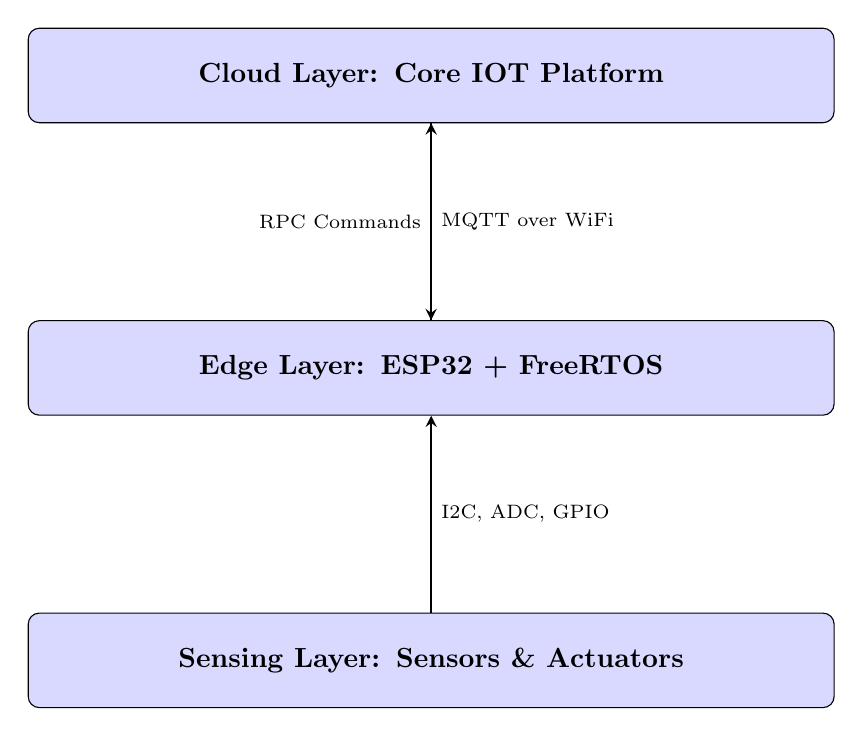
\begin{tikzpicture}[node distance=2.5cm, auto,
        layer/.style={rectangle, draw, fill=blue!15, text width=10cm, text centered, rounded corners, minimum height=1.2cm, font=\bfseries},
        component/.style={rectangle, draw, fill=green!10, text width=2.2cm, text centered, rounded corners, minimum height=0.8cm, font=\small},
        arrow/.style={->, >=stealth, thick}]
        
        % Layers
        \node[layer] (cloud) {Cloud Layer: Core IOT Platform};
        \node[layer, below=of cloud] (edge) {Edge Layer: ESP32 + FreeRTOS};
        \node[layer, below=of edge] (sensing) {Sensing Layer: Sensors \& Actuators};
        
        % Arrows
        \draw[arrow] (sensing) -- node[right, font=\scriptsize] {I2C, ADC, GPIO} (edge);
        \draw[arrow] (edge) -- node[right, font=\scriptsize] {MQTT over WiFi} (cloud);
        \draw[arrow, dashed] (cloud) -- node[left, font=\scriptsize] {RPC Commands} (edge);
        
    \end{tikzpicture}
    \caption{Three-tier system architecture showing data flow from sensors to cloud platform.}
    \label{fig:system_architecture}
\end{figure}

\section{Sensor and Actuator Integration}

We integrated multiple environmental sensors to provide comprehensive monitoring capabilities. Each sensor communicates with the ESP32 using appropriate interfaces based on its electrical characteristics and data rate requirements.

\subsection{Communication Interfaces Overview}

\subsubsection{Inter-Integrated Circuit (I2C)}
The I2C protocol is a synchronous, multi-master, multi-slave packet switched computer bus. It uses two bidirectional open-drain lines: Serial Data Line (SDA) and Serial Clock Line (SCL). We utilize I2C for the OLED display integration because it allows multiple devices to share the same bus using unique 7-bit addresses. The ESP32 acts as the master device, generating the clock signal and initiating data transfers to the SSD1306 OLED driver (address 0x3C).

\subsubsection{Analog-to-Digital Conversion (ADC)}
For analog sensors like the photoresistor and soil moisture probe, we utilize the ESP32's internal Successive Approximation Register (SAR) ADC. The ADC converts continuous analog voltage signals (0--3.3V) into discrete digital values (0--4095), enabling the microcontroller to process physical environmental parameters.

\subsection{Temperature and Humidity Sensor}

For temperature and humidity measurements, we selected the DHT11 digital sensor, which provides calibrated output through a single-wire digital interface. The DHT11 is a cost-effective sensor suitable for basic environmental monitoring applications, offering reasonable accuracy (\textpm 2\textdegree C for temperature, \textpm 5\% for humidity) with a simple communication protocol.

The DHT11 communicates using a proprietary single-wire protocol where both data transmission and power can be shared over a single GPIO pin. We connected the sensor's data pin to \texttt{GPIO 6} (labeled D4-D3 on the YoloUNO board) and utilized the Adafruit DHT library, which handles the timing-critical bit-level communication protocol automatically.

The sensor provides 8-bit resolution for both temperature (0--50\textdegree C range) and relative humidity (20--90\% range). Each measurement cycle takes approximately 2 seconds due to the sensor's internal sampling rate limitation. We configured the sensor as follows:

\begin{lstlisting}[language=C++, caption={DHT11 sensor configuration and pin definition}]
#include <DHT.h>

#define DHTPIN 6        // GPIO 6 (D4-D3 port)
#define DHTTYPE DHT11   // Sensor type specification

DHT dht(DHTPIN, DHTTYPE);
\end{lstlisting}

In our main monitoring task, we initialize the sensor and implement a polling loop with validation to ensure data integrity:

\begin{lstlisting}[language=C++, caption={DHT11 sensor reading with validation}]
void temp_humi_oled(void *pvParameters) {
    Serial.println("[OLED] Task started");
    
    // Initialize DHT11 sensor
    dht.begin();
    
    SensorData_t sensorData = {0};
    bool sensorReady = false;
    
    while (1) {
        // Read sensor values
        float humidity = dht.readHumidity();
        float temperature = dht.readTemperature();
        
        // Validate readings (check for NaN and reasonable ranges)
        bool validReading = !isnan(temperature) && !isnan(humidity) && 
                           temperature > 0 && temperature < 80 &&
                           humidity > 0 && humidity <= 100;
        
        if (!validReading) {
            vTaskDelay(pdMS_TO_TICKS(500));
            continue;  // Skip this cycle
        }
        
        if (!sensorReady) {
            sensorReady = true;
            Serial.println("[OLED] Sensor ready");
        }
        
        // Update shared data structure
        sensorData.temperature = temperature;
        sensorData.humidity = humidity;
        sendSensorData(&sensorData);
        
        // DHT11 requires minimum 1 second between readings
        vTaskDelay(pdMS_TO_TICKS(1000));
    }
}
\end{lstlisting}

The validation logic filters out erroneous readings that occasionally occur during startup or when electromagnetic interference affects the single-wire communication. We verify that values are not NaN (Not-a-Number) and fall within physically plausible ranges before accepting them. The 1-second delay between readings respects the DHT11's maximum sampling rate while providing adequate temporal resolution for environmental monitoring.

\subsection{Light Intensity Sensor}

Light intensity measurement utilizes a photoresistor (Light Dependent Resistor) coupled with an LMV358 operational amplifier to enhance signal quality. The photoresistor exhibits a nonlinear resistance characteristic that varies inversely with illumination: high resistance (several megaohms) in darkness and low resistance (hundreds of ohms) under bright light.

The LMV358 op-amp is configured as a voltage follower to buffer the signal and provide a low-impedance source for the ESP32's Analog-to-Digital Converter (ADC). The ESP32 features a 12-bit SAR ADC with a voltage range of 0--3.3V, yielding a theoretical resolution of 0.8 mV per step. However, the ADC exhibits significant nonlinearity at the extremes of its range, so we constrained our measurements to the more linear mid-range region.

We connected the sensor output to \texttt{GPIO\_NUM\_1} (labeled A2-A1 on the YoloUNO board) and implemented an exponential mapping algorithm to convert the raw ADC values to lux units:

\begin{lstlisting}[language=C++, caption={Light sensor with exponential lux conversion and smoothing filter}]
#define LIGHT_SENSOR_PIN GPIO_NUM_1
#define LUX_MIN 1.0f
#define LUX_MAX 65000.0f
#define ADC_DARK 100
#define ADC_BRIGHT 4000

void sensor_light_task(void *pvParameters) {
    pinMode(LIGHT_SENSOR_PIN, INPUT);
    
    float smoothedLux = 0;
    const float ALPHA = 0.3f;  // Smoothing coefficient
    bool firstReading = true;
    
    while (1) {
        int rawValue = analogRead(LIGHT_SENSOR_PIN);
        int constrainedADC = constrain(rawValue, ADC_DARK, ADC_BRIGHT);
        
        // Normalize to [0, 1] range
        float normalized = (float)(constrainedADC - ADC_DARK) / 
                          (ADC_BRIGHT - ADC_DARK);
        
        // Exponential mapping to lux scale
        float luxEstimate = LUX_MIN * pow(LUX_MAX / LUX_MIN, normalized);
        
        // Exponential moving average filter
        if (firstReading) {
            smoothedLux = luxEstimate;
            firstReading = false;
        } else {
            smoothedLux = ALPHA * luxEstimate + (1.0f - ALPHA) * smoothedLux;
        }
        
        float finalLux = round(smoothedLux);
        updateSensorField_Light(finalLux);
        
        vTaskDelay(pdMS_TO_TICKS(1000));
    }
}
\end{lstlisting}

The exponential mapping function accommodates the wide dynamic range of illumination levels encountered in real-world environments, spanning from moonlight (~1 lux) to direct sunlight (>100,000 lux). The exponential moving average (EMA) filter reduces noise and transient fluctuations with minimal computational overhead.

\subsection{Soil Moisture Sensor}

Soil moisture monitoring employs a capacitive moisture sensor connected to \texttt{GPIO\_NUM\_8}. Unlike resistive sensors that suffer from corrosion due to electrolysis, capacitive sensors measure the dielectric constant of the soil, which correlates with water content. The sensor outputs an analog voltage proportional to moisture level.

We configured the sensor pin as an analog input and implemented a linear mapping from the 12-bit ADC range to a percentage scale:

\begin{lstlisting}[language=C++, caption={Capacitive soil moisture sensor implementation}]
#define MOISTURE_SENSOR_PIN GPIO_NUM_8

void sensor_moisture_task(void *pvParameters) {
    pinMode(MOISTURE_SENSOR_PIN, INPUT);
    
    while (1) {
        int rawValue = analogRead(MOISTURE_SENSOR_PIN);
        
        // Convert to percentage (inverted: high ADC = dry, low ADC = wet)
        float moistureLevel = 100.0 - ((rawValue / 4095.0) * 100.0);
        
        updateSensorField_Moisture(moistureLevel);
        
        vTaskDelay(pdMS_TO_TICKS(1000));
    }
}
\end{lstlisting}

The inversion is necessary because the sensor outputs high voltage in air (dry condition) and lower voltage when immersed in water (wet condition). This configuration provides an intuitive percentage where 0\% represents completely dry soil and 100\% represents saturation.

\subsection{Flame Detection Sensor}

Fire detection capability is provided by an infrared flame sensor (KY-026 module) connected to GPIO pin 10. The sensor incorporates an IR photodiode tuned to detect the specific wavelength emitted by flames (approximately 760--1100 nm). The module includes an onboard comparator that generates a digital HIGH signal under normal conditions and transitions to LOW when flame radiation is detected.

To eliminate false triggers from transient electromagnetic interference or brief reflections, we implemented a debouncing algorithm requiring three consecutive positive detections before confirming a fire event:

\begin{lstlisting}[language=C++, caption={Flame sensor with debouncing and state machine}]
#define FLAME_SENSOR_PIN 10
#define FLAME_DEBOUNCE_COUNT 3
#define FLAME_THRESHOLD 1500

void sensor_flame_task(void *pvParameters) {
    pinMode(FLAME_SENSOR_PIN, INPUT);
    
    bool confirmedFlameState = false;
    int flameCounter = 0;
    int noFlameCounter = 0;
    
    while (1) {
        int rawValue = analogRead(FLAME_SENSOR_PIN);
        bool currentReading = (rawValue < FLAME_THRESHOLD);
        
        // Debounce logic
        if (currentReading) {
            flameCounter++;
            noFlameCounter = 0;
            if (flameCounter >= FLAME_DEBOUNCE_COUNT && !confirmedFlameState) {
                confirmedFlameState = true;
                Serial.printf("[Flame] FIRE DETECTED! (raw: %d)\n", rawValue);
                updateSystemState(STATE_FIRE_ALERT);
            }
        } else {
            noFlameCounter++;
            flameCounter = 0;
            if (noFlameCounter >= FLAME_DEBOUNCE_COUNT && confirmedFlameState) {
                confirmedFlameState = false;
                Serial.printf("[Flame] Fire cleared (raw: %d)\n", rawValue);
            }
        }
        
        updateSensorField_Flame(confirmedFlameState);
        vTaskDelay(pdMS_TO_TICKS(300));
    }
}
\end{lstlisting}

This state machine approach ensures high reliability by requiring sustained detection before triggering an alarm. The 300 ms sampling interval provides rapid response while maintaining adequate noise immunity.

\subsection{Actuator Configuration}

Our system controls three actuators for automated environmental management: a cooling fan, an RGB LED strip, and a water pump. Each actuator is controlled through GPIO pins configured as digital outputs, but with distinct control logic.

The cooling fan connects to GPIO 2 and is activated in response to elevated temperature readings or manual commands from the dashboard. We drive the fan using a simple digital ON/OFF control strategy implemented through the RPC callback mechanism described in Section~\ref{sec:data_transmission}.

The RGB LED strip (NeoPixel) is driven by a dedicated task that modulates color and brightness based on humidity levels, as detailed in Chapter 3.

The water pump implementation is more complex, featuring a dual-mode control system:
\begin{itemize}
    \item \textbf{Automatic Mode:} The pump operates based on soil moisture feedback with hysteresis control. It activates when moisture drops below 30\% (dry threshold) and deactivates only when moisture exceeds 60\% (wet threshold). This hysteresis prevents rapid cycling (chattering) of the pump relay when moisture levels fluctuate near a single threshold.
    \item \textbf{Manual Mode:} Users can override automatic control via the dashboard. When a manual command is received, the system enters manual mode for a fixed duration (5 minutes) before reverting to automatic operation. This safety timeout prevents the pump from running indefinitely if the user forgets to turn it off.
\end{itemize}

\begin{lstlisting}[language=C++, caption={Water pump control logic with hysteresis and manual override}]
if (manualModeActive) {
    // Manual override from dashboard
    pumpState = manualPumpState;
    if (millis() > manualModeTimeout) {
        manualModeActive = false; // Revert to AUTO after timeout
    }
} else {
    // Automatic hysteresis control
    if (moisture < 30.0 && !pumpState) {
        pumpState = true;  // Turn ON
    } 
    else if (moisture > 60.0 && pumpState) {
        pumpState = false; // Turn OFF
    }
}
digitalWrite(WATER_PUMP_PIN, pumpState ? HIGH : LOW);
\end{lstlisting}

\section{Data Transmission to Core IOT Platform}
\label{sec:data_transmission}

After acquiring and processing sensor data locally on the ESP32, we transmit the information to the Core IOT cloud platform for storage, analysis, and visualization. This section details the connection establishment, data serialization, and transmission protocols employed.

\subsection{MQTT Protocol Overview}

We selected the Message Queuing Telemetry Transport (MQTT) protocol for all device-to-cloud communication. MQTT is an ISO standard (ISO/IEC 20922) publish-subscribe messaging protocol designed specifically for constrained devices and unreliable networks. The protocol operates on a client-server architecture where the Core IOT platform functions as the MQTT broker and our ESP32 device acts as a client.

MQTT offers several advantages for IoT applications: minimal protocol overhead (as low as 2 bytes per message), built-in Quality of Service (QoS) levels for guaranteed delivery, and persistent session support for intermittent connectivity scenarios. The publish-subscribe model decouples data producers from consumers, allowing scalable architectures where multiple devices and services can interact without explicit peer-to-peer connections.

\subsection{Connection Establishment and Authentication}

We initialize the MQTT client using the ThingsBoard Arduino SDK, which provides a high-level abstraction over the lower-level PubSubClient library. The connection sequence begins after the WiFi task signals successful network association through a FreeRTOS binary semaphore:

\begin{lstlisting}[language=C++, caption={MQTT client initialization and ThingsBoard connection}]
constexpr uint32_t MAX_MESSAGE_SIZE = 1024U;

WiFiClient wifiClient;
Arduino_MQTT_Client mqttClient(wifiClient);
ThingsBoard tb(mqttClient, MAX_MESSAGE_SIZE);

void CORE_IOT_task(void *pvParameters) {
    // Wait for WiFi connectivity
    while (1) {
        if (xSemaphoreTake(xBinarySemaphoreInternet, portMAX_DELAY)) {
            Serial.println("[CoreIOT] WiFi ready");
            break;
        }
        vTaskDelay(500 / portTICK_PERIOD_MS);
    }
    
    // Verify token configuration
    if (CORE_IOT_TOKEN.isEmpty()) {
        Serial.println("[CoreIOT] Token not configured");
        vTaskDelete(NULL);
        return;
    }
    
    unsigned long lastPublish = 0;
    const unsigned long PUBLISH_INTERVAL = 10000;  // 10 seconds
    SensorData_t sensorData = {0};
    
    while (1) {
        CORE_IOT_reconnect();
        
        if (millis() - lastPublish >= PUBLISH_INTERVAL) {
            lastPublish = millis();
            getSensorData(&sensorData);
            
            if (tb.connected()) {
                tb.sendTelemetryData("temperature", sensorData.temperature);
                tb.sendTelemetryData("humidity", sensorData.humidity);
                tb.sendTelemetryData("light", sensorData.light_level);
                tb.sendTelemetryData("moisture", sensorData.moisture_level);
                tb.sendTelemetryData("flame", sensorData.flame_detected ? 1 : 0);
            }
        }
        vTaskDelay(500 / portTICK_PERIOD_MS);
    }
}
\end{lstlisting}

The \texttt{CORE\_IOT\_reconnect()} function handles both initial connection and automatic reconnection after network disruptions:

\begin{lstlisting}[language=C++, caption={MQTT reconnection logic with authentication and subscription}]
void CORE_IOT_reconnect() {
    if (CORE_IOT_TOKEN.isEmpty() || CORE_IOT_SERVER.isEmpty())
        return;
    
    if (!tb.connected()) {
        if (!tb.connect(CORE_IOT_SERVER.c_str(), 
                        CORE_IOT_TOKEN.c_str(), 
                        CORE_IOT_PORT))
            return;
        
        Serial.println("[CoreIOT] Connected");
        
        // Send device metadata as attributes
        tb.sendAttributeData("macAddress", WiFi.macAddress().c_str());
        tb.sendAttributeData("localIp", WiFi.localIP().toString().c_str());
        
        // Subscribe to RPC callbacks for remote control
        tb.RPC_Subscribe(callbacks.cbegin(), callbacks.cend());
    } else {
        tb.loop();  // Process incoming messages
    }
}
\end{lstlisting}

Authentication occurs through a device-specific access token provisioned during device registration on the Core IOT portal. The token serves as both the MQTT username and the authorization credential, eliminating the need for separate password authentication. Upon successful connection, we transmit the device's MAC address and local IP address as attributes, enabling network diagnostics through the dashboard.

\subsection{Telemetry Data Publishing}

Telemetry data is published at a fixed interval of 10 seconds to balance timeliness with network efficiency. The ThingsBoard SDK automatically serializes the data into JSON format and publishes it to the appropriate MQTT topic. For example, when we call \texttt{tb.sendTelemetryData("temperature", 28.5)}, the SDK constructs a JSON payload similar to:

\begin{verbatim}
{"temperature": 28.5}
\end{verbatim}

This payload is then published to the topic \texttt{v1/devices/me/telemetry}, where the broker routes it to all subscribed clients and persists it in the time-series database. Figure~\ref{fig:coreiot_telemetry} shows the Core IOT dashboard displaying real-time telemetry data from our device.

\begin{figure}[H]
    \centering
    % TODO: Replace with actual screenshot from Core IOT
    \fbox{\parbox{0.9\textwidth}{\centering
        \vspace{2cm}
        \textit{[Insert screenshot of Core IOT dashboard showing telemetry widgets]}\\
        \textit{Temperature gauge, humidity chart, light sensor, moisture level}\\
        \vspace{2cm}
    }}
    \caption{Core IOT dashboard visualizing real-time sensor telemetry data.}
    \label{fig:coreiot_telemetry}
\end{figure}

To verify that data is being received correctly by the platform, we accessed the \textit{Latest Telemetry} tab within the device details page. This interface provides a real-time view of all telemetry keys and their most recent values, along with timestamps indicating when each value was last updated. Figure~\ref{fig:coreiot_signals} demonstrates the signal verification interface.

\begin{figure}[H]
    \centering
    % TODO: Replace with actual screenshot from Core IOT
    \fbox{\parbox{0.9\textwidth}{\centering
        \vspace{2cm}
        \textit{[Insert screenshot of Core IOT Latest Telemetry panel]}\\
        \textit{Showing temperature, humidity, light, moisture, flame keys with values and timestamps]}\\
        \textit{Connection status: MQTT Connected}\\
        \vspace{2cm}
    }}
    \caption{Core IOT Latest Telemetry panel confirming successful data transmission.}
    \label{fig:coreiot_signals}
\end{figure}

This verification step is critical during development to ensure that the JSON keys defined in the firmware match exactly with the keys configured in the dashboard widgets. Any mismatch results in widgets displaying \textit{No data} even when the device is successfully transmitting.

\subsection{Bidirectional Communication: Remote Procedure Calls}

Beyond passive telemetry transmission, we implemented bidirectional communication using ThingsBoard's Remote Procedure Call (RPC) mechanism. This allows the dashboard to invoke functions on the device, enabling remote control of actuators. We registered callback functions for each controllable actuator:

\begin{lstlisting}[language=C++, caption={RPC callback registration and implementation}]
// Callback array registered with ThingsBoard SDK
const std::array<RPC_Callback, 6U> callbacks = {
    RPC_Callback{"setFanStatus", setFanStatus},
    RPC_Callback{"setLedEnabled", setLedEnabled},
    RPC_Callback{"setWaterPumpStatus", setWaterPumpStatus},
    RPC_Callback{"getFanStatus", getFanStatus},
    RPC_Callback{"getLedStatus", getLedStatus},
    RPC_Callback{"getWaterPumpStatus", getWaterPumpStatus}
};

// Example RPC callback for fan control
RPC_Response setFanStatus(const RPC_Data &data) {
    bool newState = data;
    fanEnabled = newState;
    
    // Control hardware GPIO
    pinMode(2, OUTPUT);
    digitalWrite(2, newState ? HIGH : LOW);
    
    // Update shared sensor data structure
    updateSensorField_Fan(newState);
    
    Serial.printf("[CoreIOT] Fan: %s\n", newState ? "ON" : "OFF");
    
    // Return acknowledgment
    return RPC_Response("setFanStatus", newState);
}
\end{lstlisting}

When a user toggles a switch on the dashboard, the Core IOT server publishes an RPC request to the topic \texttt{v1/devices/me/rpc/request/\$request\_id}. The SDK receives this message, deserializes the JSON payload, locates the corresponding callback function by name, and invokes it with the supplied parameters. The callback executes the hardware control action and returns an \texttt{RPC\_Response} object, which the SDK serializes and publishes back to the server. This acknowledgment is crucial; without it, the dashboard switch would timeout and revert to its previous state.

\section{Communication Protocol Analysis}

\subsection{Protocol Stack}

Our system employs a four-layer protocol stack for device-to-cloud communication:

\begin{enumerate}
    \item \textbf{Physical Layer}: IEEE 802.11 b/g/n WiFi operating in the 2.4 GHz ISM band
    \item \textbf{Network Layer}: Internet Protocol version 4 (IPv4) with DHCP for address configuration
    \item \textbf{Transport Layer}: Transmission Control Protocol (TCP) on port 1883
    \item \textbf{Application Layer}: MQTT version 3.1.1 with ThingsBoard extensions
\end{enumerate}

We chose TCP as the transport protocol rather than UDP to ensure reliable, ordered delivery of messages. While TCP introduces higher latency due to connection establishment and acknowledgment overhead, it guarantees that no telemetry packets are silently dropped. For our application, where sensor readings are transmitted at 10-second intervals, the additional latency (typically <100 ms on a local network) is negligible.

\subsection{Data Format and Serialization}

All telemetry data is serialized using JSON (JavaScript Object Notation), a human-readable text format that balances ease of debugging with reasonable compactness. The ThingsBoard SDK handles serialization automatically, but for clarity, we examine the structure of a typical telemetry message:

\begin{lstlisting}[language=json, caption={Example JSON payload transmitted to Core IOT}]
{
  "temperature": 28.5,
  "humidity": 65.2,
  "light": 850.0,
  "moisture": 45.0,
  "flame": 0,
  "fanStatus": 1,
  "neoLedEnabled": 1,
  "waterPumpStatus": 0
}
\end{lstlisting}

The MQTT protocol wraps this JSON payload with minimal overhead: a fixed header (2 bytes), variable header containing topic information, and the payload itself. For our typical message with eight key-value pairs, the total MQTT packet size ranges from 150--200 bytes, which is well within the ESP32's available memory and the network's MTU (Maximum Transmission Unit).

\subsection{Quality of Service Configuration}

MQTT supports three QoS levels:
\begin{itemize}
    \item \textbf{QoS 0 (At most once)}: Fire-and-forget delivery with no acknowledgment
    \item \textbf{QoS 1 (At least once)}: Acknowledged delivery, possible duplicates
    \item \textbf{QoS 2 (Exactly once)}: Four-way handshake guarantees single delivery
\end{itemize}

We configured our telemetry transmissions with QoS 0 to minimize network traffic and broker load. For environmental monitoring, occasional message loss is acceptable because subsequent readings provide redundancy. However, for critical RPC commands controlling actuators, the ThingsBoard SDK internally uses QoS 1 to ensure delivery while avoiding the complexity of QoS 2.

\section{Thread-Safe Data Management}

A critical aspect of our implementation is ensuring thread safety when multiple FreeRTOS tasks access shared sensor data. We defined a centralized data structure to hold all sensor readings:

\begin{lstlisting}[language=C++, caption={Sensor data structure and thread-safe access pattern}]
typedef struct {
    float temperature;
    float humidity;
    float light_level;
    float moisture_level;
    bool flame_detected;
    bool fan_enabled;
    bool neoled_enabled;
    bool water_pump_enabled;
} SensorData_t;

// Global primitives
QueueHandle_t xSensorDataQueue = NULL;
SemaphoreHandle_t xQueueMutex = NULL;

// Thread-safe field update function
void updateSensorField_Temperature(float value) {
    if (xSemaphoreTake(xQueueMutex, pdMS_TO_TICKS(50)) == pdTRUE) {
        SensorData_t data;
        if (xQueuePeek(xSensorDataQueue, &data, 0) == pdTRUE) {
            data.temperature = value;
            xQueueOverwrite(xSensorDataQueue, &data);
        }
        xSemaphoreGive(xQueueMutex);
    }
}

// Thread-safe data retrieval
bool getSensorData(SensorData_t *data) {
    bool success = false;
    if (xSemaphoreTake(xQueueMutex, pdMS_TO_TICKS(100)) == pdTRUE) {
        success = (xQueuePeek(xSensorDataQueue, data, 0) == pdTRUE);
        xSemaphoreGive(xQueueMutex);
    }
    return success;
}
\end{lstlisting}

We employ a combination of FreeRTOS queue and mutex primitives to coordinate access. The queue stores a single instance of \texttt{SensorData\_t} using the overwrite strategy, ensuring that sensor tasks always write the most recent value without blocking. The mutex serializes access to the queue operations themselves, preventing race conditions when multiple tasks attempt simultaneous updates.

This design pattern provides several benefits: it eliminates the risk of reading partially-updated structures (torn reads), ensures that the Core IOT task always transmits a consistent snapshot of all sensor values, and allows sensor tasks to operate independently at their natural update rates without explicit synchronization between sensors.




% ==================== CHAPTER 3: Task 2 - NeoPixel LED Control Based on Humidity ====================
\chapter{FreeRTOS Task Synchronization and Visual Feedback}

In this chapter, we describe the implementation of three real-time tasks that provide visual feedback based on sensor readings. We used FreeRTOS semaphores and queues to eliminate global variables and ensure thread-safe communication between tasks. The three tasks handle LED blinking based on temperature, NeoPixel color control based on humidity, and OLED display management with multiple states.

\section{Theoretical Background: Real-Time Synchronization}

In a multitasking environment like FreeRTOS, tasks often need to share resources or communicate with each other. Without proper synchronization, this can lead to race conditions (where two tasks modify data simultaneously) and data corruption. We employ three key FreeRTOS primitives to manage this complexity: Binary Semaphores, Mutexes, and Message Queues.

\subsection{Binary Semaphores for Signaling}
A Binary Semaphore can be visualized as a flag that can be either '0' (Empty) or '1' (Full). It is primarily used for **task synchronization** and **deferred interrupt processing**.

\begin{itemize}
    \item \textbf{Mechanism:} When Task A completes a job (e.g., detecting a fire), it "Gives" the semaphore (sets flag to 1). Task B, which was waiting for this event, attempts to "Take" the semaphore.
    \item \textbf{Blocking State:} Crucially, if the semaphore is empty, Task B enters the \textbf{Blocked} state. In this state, Task B consumes \textbf{zero CPU cycles}. The FreeRTOS scheduler suspends Task B and runs other lower-priority tasks. When Task A gives the semaphore, the scheduler immediately wakes up Task B, moving it to the \textbf{Ready} state.
    \item \textbf{Application in Our System:} We use binary semaphores to represent system states (\texttt{Normal}, \texttt{Warning}, \texttt{Critical}, \texttt{Fire}). The LED and OLED tasks block on these semaphores. This is far more efficient than a "busy-wait" loop that constantly checks a global variable.
\end{itemize}

\subsection{Mutexes for Resource Protection}
A Mutex (Mutual Exclusion) is a special type of binary semaphore designed specifically for protecting shared resources, such as the I2C bus or a shared data structure.

\begin{itemize}
    \item \textbf{Token Passing:} A mutex acts like a token. A task must "Take" the token before accessing the resource and "Give" it back when finished. If another task holds the token, the requesting task blocks until it becomes available.
    \item \textbf{Priority Inheritance:} Unlike standard semaphores, FreeRTOS mutexes implement \textit{Priority Inheritance}. If a high-priority task (Task H) blocks waiting for a mutex held by a low-priority task (Task L), Task L temporarily inherits Task H's priority. This prevents **Priority Inversion**, a scenario where a medium-priority task could preempt Task L, indefinitely blocking Task H.
    \item \textbf{Application in Our System:} We use \texttt{xI2CMutex} to coordinate access to the OLED display (shared between the OLED task and setup routines) and \texttt{xWaterPumpMutex} to prevent conflicts between the automatic irrigation logic and manual web control.
\end{itemize}

\subsection{Message Queues for Inter-Task Communication}
Queues provide a thread-safe way to send data structures between tasks. Unlike global variables, queues copy data by value into their own storage buffer. This ensures that the consumer receives a valid snapshot of the data even if the producer overwrites its local variable immediately after sending. This creates a robust, decoupled "Producer-Consumer" architecture.

\section{Task Layout Overview}

We implemented a producer-consumer architecture where sensor reading tasks send data to a FreeRTOS queue, and actuator control tasks read from this queue to control visual indicators. We used binary semaphores to signal system states (Normal, Warning, Critical, Fire Alert) and a mutex-protected queue to pass sensor data between tasks.

This design removes the need for global variables by storing all shared data in RTOS queues and semaphores. The queue holds the sensor readings, and semaphores signal when the system state changes. Figure~\ref{fig:task_architecture} shows how tasks communicate with each other.

\begin{figure}[H]
    \centering
    \resizebox{0.75\textwidth}{!}{
    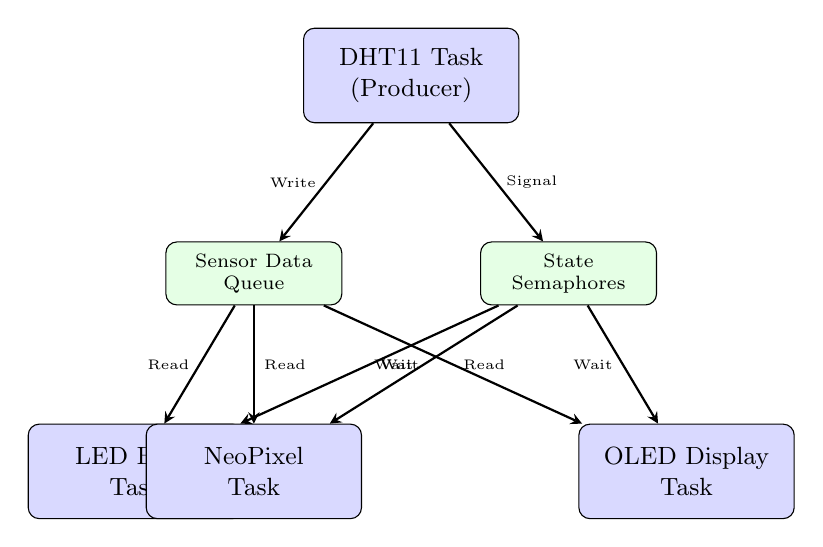
\begin{tikzpicture}[node distance=2cm, auto,
        task/.style={rectangle, draw, fill=blue!15, text width=2.5cm, text centered, rounded corners, minimum height=1.2cm, font=\small},
        data/.style={rectangle, draw, fill=green!10, text width=2cm, text centered, rounded corners, minimum height=0.8cm, font=\scriptsize},
        arrow/.style={->, >=stealth, thick}]
        
        % Producer tasks (top)
        \node[task] (sensor) {DHT11 Task\\(Producer)};
        
        % Shared resources (middle)
        \node[data, below left=1.5cm and -0.5cm of sensor] (queue) {Sensor Data\\Queue};
        \node[data, below right=1.5cm and -0.5cm of sensor] (semaphores) {State\\Semaphores};
        
        % Consumer tasks (bottom)
        \node[task, below left=1.5cm and -1cm of queue] (led) {LED Blink\\Task};
        \node[task, below=1.5cm of queue] (neo) {NeoPixel\\Task};
        \node[task, below right=1.5cm and -1cm of semaphores] (lcd) {OLED Display\\Task};
        
        % Arrows
        \draw[arrow] (sensor) -- node[left, font=\tiny] {Write} (queue);
        \draw[arrow] (sensor) -- node[right, font=\tiny] {Signal} (semaphores);
        \draw[arrow] (queue) -- node[left, font=\tiny] {Read} (led);
        \draw[arrow] (queue) -- node[right, font=\tiny] {Read} (neo);
        \draw[arrow] (queue) -- node[right, font=\tiny] {Read} (lcd);
        \draw[arrow] (semaphores) -- node[right, font=\tiny] {Wait} (led);
        \draw[arrow] (semaphores) -- node[left, font=\tiny] {Wait} (neo);
        \draw[arrow] (semaphores) -- node[left, font=\tiny] {Wait} (lcd);
    \end{tikzpicture}
    }
    \caption{Task synchronization architecture showing producer-consumer pattern with queue and semaphore-based communication.}
    \label{fig:task_architecture}
\end{figure}

\subsection{Sensors and Actuators Used}

Table~\ref{tab:sensor_actuator_overview} summarizes the main sensors and actuators that appear in this chapter. All raw readings are stored in the shared \texttt{SensorData\_t} structure and sent through the queue, while the actuator states are controlled through the LED, NeoPixel and Core IOT tasks.

\begin{table}[H]
\centering
\caption{Overview of sensors and actuators used in the visual feedback tasks.}
\label{tab:sensor_actuator_overview}
\begin{tabular}{|l|l|l|l|p{4.5cm}|}
\hline
\textbf{Type} & \textbf{Name} & \textbf{Signal} & \textbf{Unit} & \textbf{Usage in This Chapter} \\
\hline
Sensor & DHT11 Temperature & \texttt{temperature} & \textdegree C & Drives LED blink modes and OLED messages; used in state evaluation (Normal/Warning/Critical/Fire). \\
\hline
Sensor & DHT11 Humidity & \texttt{humidity} & \% & Controls NeoPixel color zones and OLED text; also part of state evaluation. \\
\hline
Sensor & Light Sensor & \texttt{light\_level} & ADC level & Logged in the queue for future use; can be shown on OLED or dashboard. Not used in current state machine. \\
\hline
Sensor & Soil Moisture Sensor & \texttt{moisture\_level} & ADC level & Logged in the queue; can be used to tune watering logic and dashboard widgets. \\
\hline
Sensor & Flame Sensor & \texttt{flame\_detected} & Boolean & Immediately forces the system into Fire Alert state; affects LED, NeoPixel and OLED emergency layouts. \\
\hline
Actuator & Normal LED & GPIO 48 & On/Off (PWM) & Indicates Normal/Warning states with different blink patterns (Task 1). \\
\hline
Actuator & Alert LED & GPIO 47 & On/Off (PWM) & Shows Critical and Fire Alert conditions (Task 1). \\
\hline
Actuator & NeoPixel RGB LED & GPIO 45 & Color + Brightness & Visualizes humidity ranges and system state (Task 2). \\
\hline
Actuator & Fan / Water Pump & Core IOT RPC & On/Off & Controlled mainly from the Core IOT dashboard; their states are still stored in \texttt{SensorData\_t} for display and logging. \\
\hline
\end{tabular}
\end{table}

\section{LED Blink Control}

\subsection{LED Behavior Summary}

We implemented a dual-LED indicator system to show environmental conditions visually. We connected two LEDs to GPIO pins 48 (normal LED) and 47 (alert LED). The blinking pattern changes based on the system state, which depends on temperature thresholds and flame detection.

The LED task responds to four distinct system states, each triggering a unique visual pattern. This multi-state design ensures that operators can assess system status at a glance without consulting the dashboard. Table~\ref{tab:led_behaviors} summarizes the complete behavior specification.

\begin{table}[H]
\centering
\caption{LED blinking behaviors mapped to system states and temperature conditions.}
\label{tab:led_behaviors}
\begin{tabular}{|l|l|l|l|l|}
\hline
\textbf{System State} & \textbf{Temperature Range} & \textbf{Normal LED (GPIO 48)} & \textbf{Alert LED (GPIO 47)} & \textbf{Blink Period} \\
\hline
Normal & 20--30\textdegree C & Slow blink (ON/OFF) & OFF & 500 ms \\
\hline
Warning & \textless 20\textdegree C or \textgreater 30\textdegree C & Slow blink & OFF & 500 ms \\
\hline
Critical & \textgreater 35\textdegree C & OFF & Fast blink & 200 ms \\
\hline
Fire Alert & Flame detected & OFF & Solid ON (max brightness) & -- \\
\hline
\end{tabular}
\end{table}

\begin{figure}[H]
    \centering
    \includegraphics[width=0.6\textwidth]{assets/led_indicator.png}
    \caption{Dual-LED indicator system showing normal LED (GPIO 48) and alert LED (GPIO 47) mounted on the YOLO Uno board.}
    \label{fig:led_indicator}
\end{figure}

\subsection{Semaphore-Based State Handling}

The temperature monitoring task evaluates sensor readings and signals the appropriate state using binary semaphores. We defined four binary semaphores corresponding to the four system states: \texttt{xSemaphoreNormal}, \texttt{xSemaphoreWarning}, \texttt{xSemaphoreCritical}, and \texttt{xSemaphoreFireAlert}.

When a state transition occurs, the monitoring task first clears all state semaphores by taking them with a zero timeout, then gives only the semaphore corresponding to the new state. This ensures that exactly one state is active at any time, preventing ambiguous conditions. The LED task can then check which semaphore is available to determine the current state.

Figure~\ref{fig:led_state_machine} illustrates the state machine governing LED behavior:

\begin{figure}[H]
    \centering
    \resizebox{0.7\textwidth}{!}{
    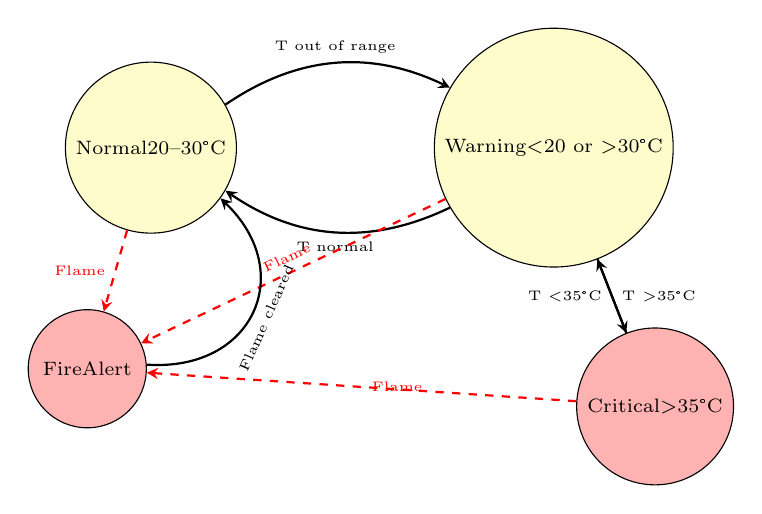
\begin{tikzpicture}[node distance=2.5cm, auto,
        state/.style={circle, draw, fill=yellow!20, text centered, minimum size=1.5cm, font=\scriptsize},
        alert/.style={circle, draw, fill=red!30, text centered, minimum size=1.5cm, font=\scriptsize},
        arrow/.style={->, >=stealth, thick}]
        
        \node[state] (normal) {Normal\\20--30\textdegree C};
        \node[state, right=of normal] (warning) {Warning\\\textless 20 or \textgreater 30\textdegree C};
        \node[alert, below right=1.5cm and -0.5cm of warning] (critical) {Critical\\\textgreater 35\textdegree C};
        \node[alert, below left=1.5cm and -0.5cm of normal] (fire) {Fire\\Alert};
        
        \draw[arrow] (normal) edge[bend left] node[above, font=\tiny] {T out of range} (warning);
        \draw[arrow] (warning) edge[bend left] node[below, font=\tiny] {T normal} (normal);
        \draw[arrow] (warning) -- node[right, font=\tiny] {T \textgreater 35\textdegree C} (critical);
        \draw[arrow] (critical) -- node[left, font=\tiny] {T \textless 35\textdegree C} (warning);
        \draw[arrow, dashed, red] (normal) -- node[left, font=\tiny] {Flame} (fire);
        \draw[arrow, dashed, red] (warning) -- node[above, font=\tiny, sloped] {Flame} (fire);
        \draw[arrow, dashed, red] (critical) -- node[right, font=\tiny] {Flame} (fire);
        \draw[arrow, bend right=70, looseness=1.5] (fire) edge node[below, font=\tiny, sloped] {Flame cleared} (normal);
    \end{tikzpicture}
    }
    \caption{State machine for LED behavior showing transitions based on temperature thresholds and flame detection.}
    \label{fig:led_state_machine}
\end{figure}

\subsection{LED Task Loop}

The LED task operates in an infinite loop, continuously monitoring the sensor queue and system state. The core logic follows this pseudocode structure:

\begin{verbatim}
TASK led_blinky():
    Initialize GPIO pins 48 and 47 as outputs
    Initialize local variables (blinkState, sensorData)
    
    WHILE TRUE:
        // Non-destructive queue read
        Peek sensor data from xSensorDataQueue
        Read current system state (thread-safe)
        
        IF state == FIRE_ALERT OR flame_detected:
            Set Alert LED to maximum brightness (GPIO 47 = HIGH)
            Set Normal LED off (GPIO 48 = LOW)
            Delay 100ms
        ELSE:
            Set Alert LED off (GPIO 47 = LOW)
            Toggle blinkState
            Set Normal LED according to blinkState
            Delay 500ms
    END WHILE
END TASK
\end{verbatim}

The task uses \texttt{xQueuePeek()} to read sensor data without removing it from the queue, so multiple tasks can read the same data. The \texttt{getSystemState()} function safely reads the current state using a mutex. We set the blink period to 500 ms, which is fast enough to catch attention but not too fast to be annoying.

The semaphore-based state checking follows this logic: the task reads sensor data from the queue using a non-destructive peek operation, then calls \texttt{getSystemState()} which internally checks which state semaphore is available. If the state is \texttt{STATE\_FIRE\_ALERT}, the alert LED is set to maximum brightness and the normal LED is turned off. Otherwise, the normal LED blinks at 500 ms intervals while the alert LED remains off.

\textbf{Role of Mutex in State Access:}
Although the LED task runs periodically using \texttt{vTaskDelay} to maintain the blink frequency, it relies on the \texttt{xStateMutex} (implied within \texttt{getSystemState}) to safely read the shared system state. This ensures that the task never reads a partially updated state or encounters a race condition if the sensor task is simultaneously transitioning the system between Normal and Warning states.

\section{Humidity NeoPixel Control}

\subsection{Humidity-to-Color Map}

We implemented a NeoPixel (WS2812B RGB LED) controller that changes color based on humidity levels. We chose colors that are easy to understand: green for good conditions, red for problems, and other colors for intermediate states.

Table~\ref{tab:humidity_colors} defines the complete humidity-to-color mapping specification:

\begin{table}[H]
\centering
\caption{NeoPixel color mapping for different humidity ranges with RGB values.}
\label{tab:humidity_colors}
\begin{tabular}{|l|l|l|l|l|}
\hline
\textbf{Humidity Range} & \textbf{Condition} & \textbf{State} & \textbf{Color} & \textbf{RGB Values} \\
\hline
\textless 30\% & Too Dry & Critical & Red & (255, 0, 0) \\
\hline
30--40\% & Dry & Warning & Orange & (255, 100, 0) \\
\hline
40--60\% & Ideal & Normal & Green & (0, 255, 0) \\
\hline
60--70\% & Acceptable & Normal & Cyan & (0, 200, 255) \\
\hline
\textgreater 70\% & Too Humid & Warning & Purple & (150, 0, 255) \\
\hline
\end{tabular}
\end{table}

We created five color zones to give more detailed feedback. The 40--60\% range shows green (ideal conditions), while other ranges show cyan (acceptable), orange (dry warning), or purple (too humid). If humidity drops below 30\%, we show red to indicate a critical condition.

\subsection{State-Based Effects}

The NeoPixel behavior changes based on the system state. In Normal state, it shows a solid color matching the humidity level. In Warning or Critical states, it blinks to catch attention. During Fire Alert, it shows solid bright red at maximum brightness, overriding all other logic.

Figure~\ref{fig:neopixel_flow} presents the decision flow implemented in the NeoPixel task:

\begin{figure}[H]
    \centering
    \resizebox{0.6\textwidth}{!}{
    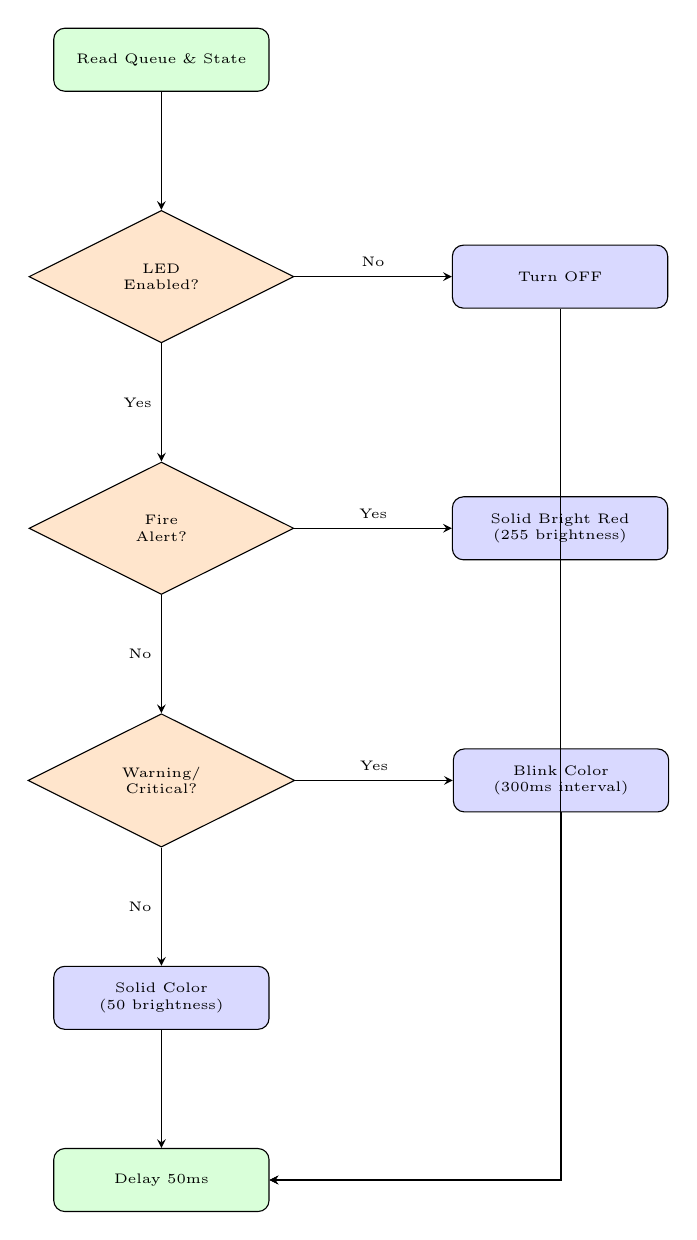
\begin{tikzpicture}[node distance=1.5cm, auto,
        decision/.style={diamond, draw, fill=orange!20, text width=2cm, text centered, aspect=2, font=\tiny},
        process/.style={rectangle, draw, fill=blue!15, text width=2.5cm, text centered, rounded corners, minimum height=0.8cm, font=\tiny},
        terminal/.style={rectangle, draw, fill=green!15, text width=2.5cm, text centered, rounded corners, minimum height=0.8cm, font=\tiny},
        arrow/.style={->, >=stealth}]
        
        \node[terminal] (start) {Read Queue \& State};
        \node[decision, below=of start] (enabled) {LED\\Enabled?};
        \node[decision, below=of enabled] (fire) {Fire\\Alert?};
        \node[decision, below=of fire] (critical) {Warning/\\Critical?};
        
        \node[process, right=2cm of enabled] (off) {Turn OFF};
        \node[process, right=2cm of fire] (fireled) {Solid Bright Red\\(255 brightness)};
        \node[process, right=2cm of critical] (blink) {Blink Color\\(300ms interval)};
        \node[process, below=of critical] (solid) {Solid Color\\(50 brightness)};
        
        \node[terminal, below=of solid] (end) {Delay 50ms};
        
        \draw[arrow] (start) -- (enabled);
        \draw[arrow] (enabled) -- node[left, font=\tiny] {Yes} (fire);
        \draw[arrow] (enabled) -- node[above, font=\tiny] {No} (off);
        \draw[arrow] (fire) -- node[left, font=\tiny] {No} (critical);
        \draw[arrow] (fire) -- node[above, font=\tiny] {Yes} (fireled);
        \draw[arrow] (critical) -- node[above, font=\tiny] {Yes} (blink);
        \draw[arrow] (critical) -- node[left, font=\tiny] {No} (solid);
        
        \draw[arrow] (off) |- (end);
        \draw[arrow] (fireled) |- (end);
        \draw[arrow] (blink) |- (end);
        \draw[arrow] (solid) -- (end);
    \end{tikzpicture}
    }
    \caption{NeoPixel control flow showing decision logic based on LED enable status and system state.}
    \label{fig:neopixel_flow}
\end{figure}

\subsection{NeoPixel Task Loop}

The NeoPixel task implements a hierarchical priority system where fire alerts override all other conditions. The pseudocode structure demonstrates this layered decision logic:

\begin{verbatim}
FUNCTION getColorByHumidity(humidity):
    IF humidity < 30: RETURN Red(255,0,0)
    ELSE IF humidity < 40: RETURN Orange(255,100,0)
    ELSE IF humidity <= 60: RETURN Green(0,255,0)
    ELSE IF humidity <= 70: RETURN Cyan(0,200,255)
    ELSE: RETURN Purple(150,0,255)
END FUNCTION

TASK neo_blinky():
    Initialize NeoPixel strip on GPIO 45
    Set default brightness to 50
    
    WHILE TRUE:
        Read sensor data from queue
        Read current system state
        
        IF LED disabled (via RPC control):
            Turn off LED
            CONTINUE
        END IF
        
        IF state == FIRE_ALERT OR flame detected:
            Set brightness to 255 (maximum)
            Display solid bright red
        ELSE IF state == WARNING OR CRITICAL:
            Set brightness based on severity (70 or 100)
            Get color from humidity mapping
            Blink color at 300ms intervals
        ELSE (Normal state):
            Set brightness to 50 (power saving)
            Get color from humidity mapping
            Display solid color
        END IF
        
        Delay 50ms
    END WHILE
END TASK
\end{verbatim}

The color selection function checks humidity ranges to pick the right color. We adjust brightness to save power during normal operation (brightness 50) and make alerts more visible (brightness 70 for warnings, 100 for critical). This makes critical states stand out even when using the same color.

The semaphore-based state checking works as follows: the task first checks if the LED is enabled via RPC control by reading from the sensor data queue. If disabled, the LED remains off. Otherwise, it calls \texttt{getSystemState()} to determine the current system state. Based on the state semaphore, the task selects the appropriate behavior: fire alert displays solid bright red at maximum brightness, warning/critical states blink the humidity-based color at 300 ms intervals, and normal state displays a solid color at reduced brightness.

\section{OLED Status Display}

\subsection{OLED Layout Modes}

We implemented an OLED display (SSD1306, 128x64 pixels) that shows environmental data with different layouts based on the system state. In Normal state, it shows detailed temperature and humidity readings. In Warning or Critical states, it highlights the problem. In Fire Alert, it shows an emergency message.

Table~\ref{tab:oled_states} enumerates the display states and their visual characteristics:

\begin{table}[H]
\centering
\caption{OLED display states with corresponding visual elements and trigger conditions.}
\label{tab:oled_states}
\begin{tabular}{|l|p{3cm}|p{4cm}|p{4cm}|}
\hline
\textbf{Display State} & \textbf{Trigger Condition} & \textbf{Visual Elements} & \textbf{Information Displayed} \\
\hline
Normal & 20--30\textdegree C and 40--70\% humidity & Clean layout, comfort status (IDEAL/GOOD), smiley icon & Full temp/humidity values, status text \\
\hline
Warning & Temperature or humidity outside normal range & Blinking border (500ms), warning message (HOT/COLD/DRY/HUMID), exclamation icon & Abbreviated readings, specific warning reason \\
\hline
Critical & Temperature \textgreater 35\textdegree C or humidity \textless 30\% & Inverted header (flashing), action message, large exclamation & Temperature, humidity, corrective action text \\
\hline
Fire Alert & Flame detected & Full screen flash (white/black), FIRE!! text, EVACUATE NOW message & Emergency alert only, no sensor data \\
\hline
\end{tabular}
\end{table}

\begin{figure}[H]
    \centering
    \includegraphics[width=0.6\textwidth]{assets/oled_display.png}
    \caption{OLED screen on the YOLO Uno board showing temperature and humidity with different layouts for each state.}
    \label{fig:oled_display_real}
\end{figure}

\subsection{State Selection Flow}

The OLED task checks which state semaphore is available to decide which display function to call. Instead of constantly checking variables, the semaphore approach lets the task wait until the state changes, which saves CPU time.

We created separate functions for each display state: \texttt{drawNormalDisplay()}, \texttt{drawWarningDisplay()}, \texttt{drawCriticalDisplay()}, and \texttt{drawFireAlertDisplay()}. This makes the code easier to maintain and test.

Figure~\ref{fig:oled_rendering} illustrates the OLED rendering pipeline:

\begin{figure}[H]
    \centering
    \resizebox{0.8\textwidth}{!}{
    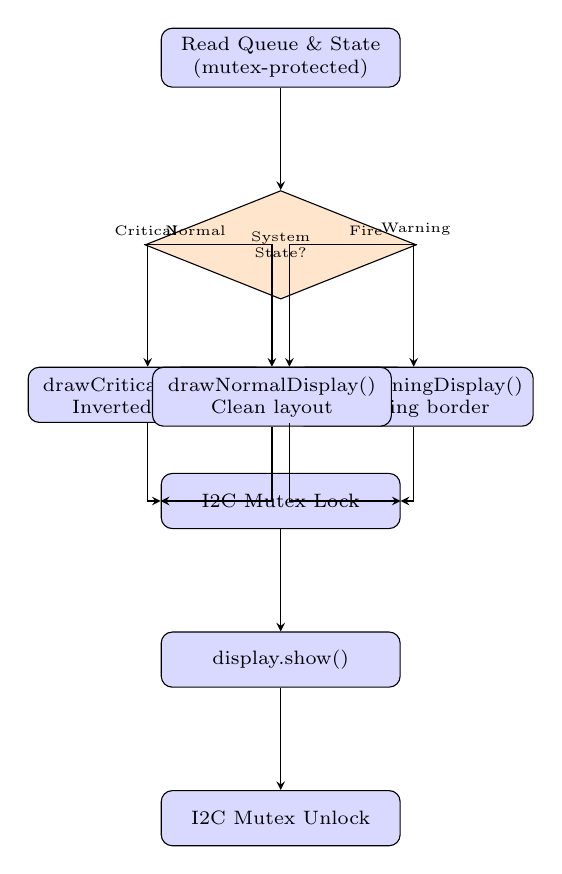
\begin{tikzpicture}[node distance=1.3cm, auto,
        process/.style={rectangle, draw, fill=blue!15, text width=2.8cm, text centered, rounded corners, minimum height=0.7cm, font=\scriptsize},
        decision/.style={diamond, draw, fill=orange!20, text width=1.8cm, text centered, aspect=2.5, font=\tiny},
        arrow/.style={->, >=stealth}]
        
        \node[process] (read) {Read Queue \& State (mutex-protected)};
        \node[decision, below=of read] (state) {System\\State?};
        
        \node[process, below left=1.2cm and -2.5cm of state] (fire) {drawFireAlertDisplay()\\Full screen flash};
        \node[process, below left=1.2cm and -0.7cm of state] (critical) {drawCriticalDisplay()\\Inverted header};
        \node[process, below right=1.2cm and -0.7cm of state] (warning) {drawWarningDisplay()\\Blinking border};
        \node[process, below right=1.2cm and -2.5cm of state] (normal) {drawNormalDisplay()\\Clean layout};
        
        \node[process, below=2.2cm of state] (i2c) {I2C Mutex Lock};
        \node[process, below=of i2c] (display) {display.show()};
        \node[process, below=of display] (unlock) {I2C Mutex Unlock};
        
        \draw[arrow] (read) -- (state);
        \draw[arrow] (state) -| node[above, font=\tiny, pos=0.2] {Fire} (fire);
        \draw[arrow] (state) -| node[above, font=\tiny, pos=0.2] {Critical} (critical);
        \draw[arrow] (state) -| node[above, font=\tiny, pos=0.2] {Warning} (warning);
        \draw[arrow] (state) -| node[above, font=\tiny, pos=0.2] {Normal} (normal);
        
        \draw[arrow] (fire) |- (i2c);
        \draw[arrow] (critical) |- (i2c);
        \draw[arrow] (warning) |- (i2c);
        \draw[arrow] (normal) |- (i2c);
        
        \draw[arrow] (i2c) -- (display);
        \draw[arrow] (display) -- (unlock);
    \end{tikzpicture}
    }
    \caption{OLED rendering pipeline showing state-based function selection and I2C mutex protection.}
    \label{fig:oled_rendering}
\end{figure}

\subsection{Queue and Semaphore Data Flow}

One of the main requirements was to remove all global variables and use RTOS primitives instead. We did this by putting all sensor readings into a \texttt{SensorData\_t} structure that goes through the queue, and using semaphores for state information.

We removed global variables in three ways:

\begin{enumerate}
    \item \textbf{Data in Queue:} All sensor values are stored in the \texttt{SensorData\_t} struct in the queue, so we don't need separate global variables for temperature, humidity, etc.
    \item \textbf{State with Semaphores:} We use binary semaphores to signal system states instead of global state variables
    \item \textbf{Task Communication:} Tasks talk to each other through queues and semaphores, not shared memory, which makes it thread-safe
\end{enumerate}

The OLED task demonstrates this pattern through its main loop structure:

\begin{verbatim}
TASK temp_humi_oled():
    Initialize OLED display (with I2C mutex protection)
    Initialize DHT11 sensor
    
    WHILE TRUE:
        Read temperature and humidity from DHT11
        Validate readings
        
        // Pack data into struct (no global variables)
        sensorData.temperature = temperature
        sensorData.humidity = humidity
        
        // Evaluate state using pure function
        newState = evaluateSystemState(temp, humidity, flame)
        
        // Update semaphores (thread-safe)
        updateSystemState(newState)
        
        // Send to queue for other tasks
        sendSensorData(sensorData)
        
        // Render display based on state
        Acquire I2C mutex
        currentState = getSystemState()
        SWITCH currentState:
            CASE FIRE_ALERT: drawFireAlertDisplay()
            CASE CRITICAL: drawCriticalDisplay()
            CASE WARNING: drawWarningDisplay()
            CASE NORMAL: drawNormalDisplay()
        Release I2C mutex
        
        // Adaptive delay based on urgency
        IF state >= WARNING: Delay 300ms
        ELSE: Delay 1000ms
    END WHILE
END TASK
\end{verbatim}

The state evaluation is implemented as a pure function with no side effects:

\begin{verbatim}
FUNCTION evaluateSystemState(temp, humidity, flame):
    IF flame: RETURN FIRE_ALERT
    IF temp > 35 OR humidity < 30: RETURN CRITICAL
    IF temp < 20 OR temp > 30 OR humidity < 40 OR humidity > 70:
        RETURN WARNING
    RETURN NORMAL
END FUNCTION
\end{verbatim}

The state update function handles semaphore signaling with mutex protection, ensuring atomic state transitions:

\begin{verbatim}
FUNCTION updateSystemState(newState):
    Acquire state mutex
    IF newState != currentState:
        // Clear all semaphores atomically
        Take all state semaphores (timeout = 0)
        
        // Give only the active state semaphore
        SWITCH newState:
            CASE NORMAL: Give xSemaphoreNormal
            CASE WARNING: Give xSemaphoreWarning
            CASE CRITICAL: Give xSemaphoreCritical
            CASE FIRE_ALERT: Give xSemaphoreFireAlert
        
        currentState = newState
    Release state mutex
END FUNCTION
\end{verbatim}

This architecture completely eliminates global variable dependencies by using FreeRTOS queues for data passing and semaphores for state signaling, achieving deterministic thread-safe inter-task communication without shared memory vulnerabilities.

The OLED task works like this: it reads temperature and humidity from the DHT sensor, checks if the readings are valid, and puts them into a \texttt{SensorData\_t} structure. This structure is sent to the queue so other tasks can read it, avoiding global variables.

To determine the system state, we call \texttt{evaluateSystemState()} which takes sensor readings and returns the state based on thresholds. This function doesn't use any global variables. Then we call \texttt{updateSystemState()} to update the semaphores.

The \texttt{updateSystemState()} function works atomically: it first takes a mutex, then clears all state semaphores by taking them with zero timeout, and finally gives only the semaphore for the new state. This way, only one state semaphore is available at a time, so other tasks can check which state is active.

For displaying, the task takes the I2C mutex before writing to the OLED, calls \texttt{getSystemState()} to check which state semaphore is available, and then calls the right display function. We use different delays: 300 ms during warnings/critical states for faster updates, and 1000 ms during normal operation to save CPU.

\section{Light Intensity Processing}

\subsection{Signal Conditioning and Conversion}

The light sensor task functions as a pure producer in our architecture. It acquires analog voltage readings from the photoresistor circuit and converts them into meaningful lux units. The conversion process is non-trivial due to the logarithmic response of the human eye and the sensor's characteristics.

We implemented a digital signal processing pipeline that includes:
\begin{itemize}
    \item \textbf{Input Constraining:} Clamping raw ADC values to the linear region of the sensor.
    \item \textbf{Exponential Mapping:} Converting linear ADC steps to a logarithmic lux scale.
    \item \textbf{Smoothing Filter:} Applying an Exponential Moving Average (EMA) to reduce measurement noise.
\end{itemize}

\subsection{Implementation Logic}

The task operates independently, publishing processed values to the shared sensor queue.

\begin{verbatim}
TASK sensor_light_task():
    Initialize ADC on GPIO 1
    Initialize smoothedLux = 0
    ALPHA = 0.3 // Smoothing factor
    
    WHILE TRUE:
        rawADC = analogRead(LIGHT_SENSOR_PIN)
        constrained = constrain(rawADC, 100, 4000)
        
        // Normalize to 0.0 - 1.0
        normalized = (constrained - 100) / 3900.0
        
        // Exponential mapping: 1 lux to 65000 lux
        luxEstimate = 1.0 * pow(65000.0, normalized)
        
        // Low-pass filter
        smoothedLux = (ALPHA * luxEstimate) + ((1 - ALPHA) * smoothedLux)
        
        // Update shared data
        updateSensorField_Light(smoothedLux)
        
        Delay 1000ms
    END WHILE
END TASK
\end{verbatim}

\section{Soil Moisture and Automated Irrigation}

\subsection{Hybrid Producer-Consumer Architecture}

The water pump task represents a hybrid producer-consumer model. It consumes moisture data from the shared queue to make control decisions (Consumer role) and produces pump status updates back to the system (Producer role).

This task manages the water pump actuator using a robust hysteresis control algorithm to prevent rapid switching cycles. It also integrates a manual override mechanism controlled via the dashboard, which requires careful synchronization using a mutex to prevent conflict between automatic logic and user commands.

\subsection{Control Logic with Safety Timeout}

The implementation prioritizes user commands but includes a safety timeout to revert to automatic mode, preventing flooding accidents.

\begin{verbatim}
TASK sensor_water_pump_task():
    Initialize Pump GPIO as OUTPUT
    Create xWaterPumpMutex
    
    WHILE TRUE:
        // Consume latest sensor data
        Get sensorData from Queue
        
        Acquire xWaterPumpMutex
        
        // Check manual mode expiration
        IF manualModeActive AND (millis() > manualTimeout):
            manualModeActive = FALSE
        
        IF manualModeActive:
            pumpState = manualState
        ELSE:
            // Auto mode with Hysteresis
            IF moisture < 30.0 AND pumpState == OFF:
                pumpState = ON
            ELSE IF moisture > 60.0 AND pumpState == ON:
                pumpState = OFF
        
        Release xWaterPumpMutex
        
        // Actuate hardware
        digitalWrite(PUMP_PIN, pumpState)
        
        // Update system status
        updateSensorField_WaterPump(pumpState)
        
        Delay 500ms
    END WHILE
END TASK
\end{verbatim}

\textbf{Mutex for Conflict Prevention:}
The \texttt{xWaterPumpMutex} plays a vital role in this task. Since the water pump can be controlled by two independent sources—the automatic logic in this task and the manual override commands from the Web Server task (via RPC)—there is a risk of conflicting write operations. The mutex ensures mutual exclusion: if the Web Server is updating the manual mode status, the automatic task must wait until that operation is complete before it can read or write the pump state. This guarantees data integrity and prevents "glitchy" actuator behavior.

\section{Critical Safety Monitoring (Flame Detection)}

\subsection{High-Priority Event Detection}

The flame detection task is assigned the highest priority in our system (Priority 4) to ensure immediate response to fire hazards. Unlike other monitoring tasks that report data periodically, this task operates as a watchdog that can trigger a system-wide state transition to \texttt{STATE\_FIRE\_ALERT}.

To prevent false alarms caused by transient infrared noise (e.g., remote controls or sunlight glint), we implemented a debouncing state machine. This requires multiple consecutive positive readings before confirming a fire event.

\subsection{Debouncing Algorithm}

The logic ensures reliability by validating the signal stability over a short time window.

\begin{verbatim}
TASK sensor_flame_task():
    Initialize Flame Sensor GPIO 10
    flameCounter = 0
    confirmedState = FALSE
    
    WHILE TRUE:
        rawVal = analogRead(FLAME_PIN)
        isFlame = (rawVal < THRESHOLD)
        
        IF isFlame:
            flameCounter++
            IF flameCounter >= 3 AND !confirmedState:
                confirmedState = TRUE
                // Critical State Transition
                updateSystemState(STATE_FIRE_ALERT)
        ELSE:
            flameCounter = 0
            IF confirmedState:
                confirmedState = FALSE
                // Clear Alert
                updateSystemState(STATE_NORMAL)
        
        // Update shared data
        updateSensorField_Flame(confirmedState)
        
        Delay 300ms // Fast sampling
    END WHILE
END TASK
\end{verbatim}


% ==================== CHAPTER 4: Task 3 - Temperature and Humidity Monitoring with LCD Display ====================
\chapter{Task 3 - Temperature and Humidity Monitoring with OLED Display}

This chapter details the design and implementation of the environmental monitoring subsystem, which integrates an OLED display for real-time data visualization. The primary objective of this task is to provide immediate, intuitive feedback on ambient conditions to the user. We designed the system to continuously monitor temperature and humidity levels and dynamically adapt the visual interface based on predefined operational states: Normal, Warning, Critical, and Fire Alert. This adaptive display strategy ensures that critical safety information is prioritized over routine data, thereby enhancing the system's usability and responsiveness in emergency scenarios.

\section{OLED Layout Modes}

We utilized an SSD1306 OLED display (128x64 pixels) to present environmental data. Rather than employing a static layout, we implemented a dynamic rendering engine that switches between four distinct display modes based on the current system state. This approach allows the system to highlight the most relevant information for each specific condition.

\subsection{Normal State}
In the \textbf{Normal} state (Temperature 15--30\textdegree C, Humidity 40--80\%), the display is configured to maximize readability of the sensor readings. We designed a clean, uncluttered layout that prominently features the current temperature and humidity values. To provide immediate reassurance to the user, the interface includes a comfort status indicator (displaying "IDEAL" or "GOOD") and a graphical smiley icon. This mode is intended for routine monitoring when environmental conditions are within safe limits.

\begin{figure}[H]
    \centering
    \includegraphics[width=0.6\textwidth]{assets/oled_normal.png}
    \caption{OLED display in Normal state showing temperature, humidity, and comfort icon.}
    \label{fig:oled_normal}
\end{figure}

\subsection{Warning State}
The \textbf{Warning} state is triggered when environmental parameters drift outside the optimal comfort range (Temperature \textless 15\textdegree C or \textgreater 33\textdegree C, or Humidity \textless 40\% or \textgreater 80\%). To attract the user's attention, we implemented a visual blinking effect on the display border with a 500ms interval. The layout shifts focus from detailed readings to specific warning messages (e.g., "HOT", "COLD", "DRY", "TOO HUMID"), accompanied by an exclamation icon. This visual hierarchy ensures that the user is promptly alerted to the deviation before conditions deteriorate further.

\subsection{Critical State}
In the \textbf{Critical} state (Temperature \textgreater 40\textdegree C or Humidity \textless 30\%), the system escalates the visual urgency. We inverted the display header colors and implemented a flashing effect to maximize contrast and visibility. The screen presents the sensor values alongside imperative corrective action messages (e.g., "TOO HOT! Cool down!" or "TOO DRY! Add moisture!"). This design is intended to guide the user toward immediate remediation steps to prevent equipment damage or health risks.

\subsection{Fire Alert State}
The \textbf{Fire Alert} state represents the highest priority condition in the system hierarchy. Upon detection of a flame by the sensor, the display logic overrides all other data to present a full-screen emergency alert. We designed this mode to display "FIRE DETECTED!" and "EVACUATE NOW" in large, bold text, ensuring that the warning is legible from a distance. In this state, routine sensor data is suppressed to prevent distraction during an emergency.

\begin{figure}[H]
    \centering
    \includegraphics[width=0.6\textwidth]{assets/oled_fire.png}
    \caption{OLED display in Fire Alert state showing emergency evacuation message.}
    \label{fig:oled_fire}
\end{figure}

\section{State Selection Flow}

To manage the transitions between these display modes, we implemented a semaphore-based control mechanism within the FreeRTOS environment. Instead of relying on complex conditional logic that polls global variables, the display task waits for specific binary semaphores that signal the current system state. This design ensures that the visual output remains strictly synchronized with the core system logic.

The state evaluation logic enforces a strict priority hierarchy: \textbf{Fire Alert} takes precedence over \textbf{Critical}, which overrides \textbf{Warning}, with \textbf{Normal} being the default state. This hierarchical approach guarantees that the most urgent information is always displayed, regardless of other concurrent conditions.

The following pseudocode illustrates the selection flow implemented in our display task:

\begin{verbatim}
FUNCTION updateDisplay():
    Acquire I2C Mutex
    
    // Check which state is active
    state = getSystemState()
    
    SWITCH state:
        CASE FIRE_ALERT:
            drawFireAlertDisplay(animationFrame)
            BREAK
            
        CASE CRITICAL:
            drawCriticalDisplay(temp, humi, animationFrame)
            BREAK
            
        CASE WARNING:
            drawWarningDisplay(temp, humi, animationState)
            BREAK
            
        CASE NORMAL:
            drawNormalDisplay(temp, humi)
            BREAK
            
    Release I2C Mutex
    
    // Adjust refresh rate based on urgency
    IF state >= WARNING:
        Delay 300ms  // Fast refresh for alerts
    ELSE:
        Delay 1000ms // Save power in normal mode
END FUNCTION
\end{verbatim}

\section{Queue and Semaphore Data Flow}

A key architectural requirement for this project was the elimination of global variables to ensure thread safety and modularity. We achieved this by encapsulating all sensor readings within a \texttt{SensorData\_t} structure, which is transmitted between tasks via FreeRTOS queues. Furthermore, system states are managed exclusively through binary semaphores.

Our implementation removes global variable dependencies through three specific mechanisms:

\begin{enumerate}
    \item \textbf{Queue-Based Data Transfer:} All sensor values are packed into the \texttt{SensorData\_t} struct and passed through a queue. This prevents race conditions associated with shared global variables.
    \item \textbf{Semaphore-Based State Signaling:} We utilize binary semaphores to signal state changes, providing a robust synchronization primitive that replaces global state flags.
    \item \textbf{Inter-Task Communication:} Tasks communicate solely through these OS primitives, ensuring that data access is thread-safe and deterministic.
\end{enumerate}

The OLED task structure demonstrates this pattern. It initializes the display and sensor, then enters an infinite loop where it reads data, evaluates the system state, updates semaphores, and renders the appropriate display layout. The state evaluation is implemented as a pure function, ensuring no side effects, while the state update function uses mutexes to guarantee atomic transitions between states.

\begin{verbatim}
TASK temp_humi_oled():
    Initialize OLED display (with I2C mutex protection)
    Initialize DHT11 sensor
    
    WHILE TRUE:
        Read temperature and humidity from DHT11
        Validate readings
        
        // Pack data into struct (no global variables)
        sensorData.temperature = temperature
        sensorData.humidity = humidity
        
        // Evaluate state using pure function
        newState = evaluateSystemState(temp, humidity, flame)
        
        // Update semaphores (thread-safe)
        updateSystemState(newState)
        
        // Send to queue for other tasks
        sendSensorData(sensorData)
        
        // Render display based on state
        Acquire I2C mutex
        currentState = getSystemState()
        SWITCH currentState:
            CASE FIRE_ALERT: drawFireAlertDisplay()
            CASE CRITICAL: drawCriticalDisplay()
            CASE WARNING: drawWarningDisplay()
            CASE NORMAL: drawNormalDisplay()
        Release I2C mutex
        
        // Adaptive delay based on urgency
        IF state >= WARNING: Delay 300ms
        ELSE: Delay 1000ms
    END WHILE
END TASK
\end{verbatim}

This architecture ensures that the display task operates independently yet synchronously with the rest of the system, providing reliable visual feedback without compromising the stability of the real-time operating system.


% ==================== CHAPTER 5: Task 4 - Web Server in Access Point Mode ====================
\chapter{Web Server Interface and Cloud Integration}

This chapter refines the web server and cloud integration so the report is accurate and presentation-ready. The ESP32 runs AP and STA together: the AP keeps local access alive for control/OTA, while STA reconnects in the background to restore cloud links and telemetry.

\section{Web Server Design}

Static UI assets live in LittleFS and are served by \texttt{ESPAsyncWebServer} so request handling stays asynchronous and non-blocking. Figure~\ref{fig:backend_block} summarizes how the networking stack, web layer, message queues, and FreeRTOS tasks interact from ingress to actuation/cloud forwarding.

\begin{figure}[H]
    \centering
    % TODO: Thay bằng sơ đồ khối backend thực tế
    \fbox{\parbox{0.9\textwidth}{\centering
        \vspace{2.0cm}
        \textit{[Backend Block Diagram]}\\
        AP/STA WiFi $\rightarrow$ ESPAsyncWebServer + WebSocket $\rightarrow$ Message Queue $\rightarrow$ FreeRTOS Tasks (Sensor, Control, Cloud) $\rightarrow$ Peripherals/Cloud\\
        \vspace{2.0cm}
    }}
    \caption{Sơ đồ khối backend: từ tầng mạng đến queue và các task điều khiển/đồng bộ cloud.}
    \label{fig:backend_block}
\end{figure}

\subsection{Access Point Configuration}

The ESP32 always boots in AP+STA mode so it never becomes unreachable. The AP is fixed at SSID \texttt{YoloUNO\_AP}, static IP \texttt{192.168.4.1}, WPA2-PSK. In \texttt{task\_wifi.cpp}, \texttt{ensureAP()} keeps that AP alive while \texttt{startSTA()} tries the stored home WiFi; if the STA link drops, \texttt{Wifi\_reconnect()} retries the uplink but still preserves the AP. Practically, users can always reach \texttt{192.168.4.1} for local control/OTA even when home WiFi changes; once STA succeeds, the device also announces its LAN IP and OTA URL.

\subsection{Request Handling and Task Flow}

All traffic enters the asynchronous web layer in \texttt{task\_webserver.cpp}. Static files, REST endpoints, and WebSocket events share a consistent path: parse/validate input, execute the requested control or info action, then broadcast the refreshed state to connected clients. Key endpoints include health check (\texttt{/health}), device info (\texttt{/info}), CSV lifecycle (\texttt{/download}, \texttt{/csv-info}, \texttt{/clear}), and OTA hooks (ElegantOTA). WebSocket messages are handled in \texttt{onEvent()} and forwarded to \texttt{handleWebSocketMessage()} for device control.

\textbf{Backend execution.} \texttt{connnectWSV()} (in \texttt{task\_webserver.cpp}) mounts LittleFS assets, registers REST/WebSocket handlers, and enables ElegantOTA before \texttt{server.begin()}. \texttt{onEvent()} parses WebSocket frames and hands them to \texttt{handleWebSocketMessage()} for LED/pump control and state fan-out. \texttt{task\_wifi.cpp} enforces AP+STA so the AP at \texttt{192.168.4.1} stays up during STA reconnects. In the cloud path, \texttt{CORE\_IOT\_task} keeps the MQTT session alive, publishes telemetry every 10s, and applies RPC commands (fan/LED/pump) while mirroring states back to keep the dashboard switches in sync. Health, info, CSV download/clear/info, and OTA progress are exposed via lightweight endpoints and WebSocket notifications.
\textbf{RPC and reconnect.} RPC callbacks (\texttt{setFanStatus}, \texttt{setLedEnabled}, \texttt{setWaterPumpStatus}) are executed inside \texttt{CORE\_IOT\_task}; each command drives the actuator, updates shared sensor state, and the paired getter RPCs return the latest value so dashboard toggles stay aligned. The MQTT loop reconnects whenever the link drops, resubscribes RPC/shared attributes, and resumes publishing without losing state. On the WiFi side, \texttt{Wifi\_reconnect()} rate-limits STA retries every 30s but never drops the AP, ensuring local UI/WebSocket/OTA remain reachable during WAN outages.

\begin{figure}[H]
    \centering
    % TODO: Replace with actual backend flowchart
    \fbox{\parbox{0.9\textwidth}{\centering
        \vspace{1.8cm}
        \textit{[Backend Flowchart]}\\
        Client HTTP/WebSocket $\rightarrow$ Async Handler $\rightarrow$ Validate/Dispatch $\rightarrow$ Control or Info Action $\rightarrow$ State Broadcast\\
        \vspace{1.8cm}
    }}
    \caption{Request/response flow across HTTP/WebSocket handlers, control actions, and outbound broadcasts.}
    \label{fig:backend_flow}
\end{figure}

\subsection{User Interface Implementation}

UI assets (HTML5/CSS3/JavaScript) are decoupled from firmware—update LittleFS only to change the look. WebSocket pushes keep WiFi/MQTT badges live without reloading the page.

\begin{enumerate}
    \item \textbf{Device Control Panel:} LED (GPIO 48) and Pump/Fan (GPIO 2) toggles.
    \item \textbf{Real-time Status:} Temperature, humidity, light level, WiFi/cloud indicators.
    \item \textbf{Cloud Sync State:} MQTT connection badge and last publish timestamp.
\end{enumerate}

\begin{figure}[H]
    \centering
    % TODO: Replace placeholder image paths with real screenshots
    \begin{minipage}{0.45\textwidth}
        \centering
        \includegraphics[width=0.9\textwidth]{assets/ui_home_placeholder.png}
        \caption*{Home — overview + quick toggles}
    \end{minipage}
    \hfill
    \begin{minipage}{0.45\textwidth}
        \centering
        \includegraphics[width=0.9\textwidth]{assets/ui_devices_placeholder.png}
        \caption*{Devices — LED/Pump controls + live metrics}
    \end{minipage}

    \vspace{0.5cm}

    \begin{minipage}{0.45\textwidth}
        \centering
        \includegraphics[width=0.9\textwidth]{assets/ui_info_placeholder.png}
        \caption*{Info — device ID, firmware, IP, uptime}
    \end{minipage}
    \hfill
    \begin{minipage}{0.45\textwidth}
        \centering
        \includegraphics[width=0.9\textwidth]{assets/ui_settings_placeholder.png}
        \caption*{Settings — WiFi credentials, MQTT token, publish interval}
    \end{minipage}
    \caption{Placeholders for UI screens: Home, Devices, Info, Settings.}
    \label{fig:web_ui_screens}
\end{figure}

\subsection{Web Communication Protocols}

\subsubsection{HTTP vs. WebSocket}
Traditional web servers use the HTTP protocol, which follows a request-response model. The client requests data, the server responds, and the connection is closed. This is inefficient for real-time control because the client must constantly poll the server to get updates.

For our control interface, we chose the \textbf{WebSocket} protocol. WebSocket provides a full-duplex communication channel over a single TCP connection. Once established, the server can push data to the client immediately without waiting for a request. This significantly reduces latency and network overhead, making it ideal for controlling actuators (like LEDs) and displaying live sensor data.

\subsection{WebSocket Communication}

To achieve real-time performance without page reloads, we utilized the WebSocket protocol. Unlike traditional HTTP polling, WebSocket establishes a persistent, full-duplex connection between the browser and the ESP32.

\begin{lstlisting}[language=C++, caption={WebSocket event handler for real-time control}]
void onEvent(AsyncWebSocket *server, AsyncWebSocketClient *client, 
             AwsEventType type, void *arg, uint8_t *data, size_t len) {
    if (type == WS_EVT_DATA) {
        AwsFrameInfo *info = (AwsFrameInfo *)arg;
        if (info->opcode == WS_TEXT) {
            String message = String((char *)data).substring(0, len);
            
            // Parse JSON command
            // Example: {"action":"toggleLed", "value":true}
            handleWebSocketMessage(message);
        }
    }
}
\end{lstlisting}

When a user clicks a button on the web interface, a JSON message is sent over the WebSocket. The ESP32 parses this message and triggers the corresponding FreeRTOS task (e.g., giving a semaphore to the LED task). Conversely, when sensor values change, the ESP32 broadcasts the new data to all connected clients immediately.

\begin{figure}[H]
    \centering
    % TODO: Replace with actual diagram of WebSocket flow
    \fbox{\parbox{0.8\textwidth}{\centering
        \vspace{1.5cm}
        \textit{[Insert diagram of WebSocket Communication Flow here]}\\
        \textit{Client -> JSON Command -> ESP32 -> Task Notification}\\
        \vspace{1.5cm}
    }}
    \caption{WebSocket communication flow for real-time device control.}
    \label{fig:websocket_flow}
\end{figure}

\section{Cloud Integration and Data Publishing}

While the local web server provides immediate control, long-term data storage and remote access are handled by the CoreIOT cloud platform.

\subsection{Station Mode Connectivity}

The device connects to the local WiFi network in Station (STA) mode. We implemented a robust reconnection state machine that:
\begin{enumerate}
    \item Attempts to connect to the configured WiFi SSID.
    \item If connection fails, it waits for a backoff period before retrying.
    \item Periodically checks connection health and triggers reconnection if the link is dropped.
    \item Synchronizes system time via NTP (Network Time Protocol) upon successful connection.
\end{enumerate}

Crucially, the reconnection logic runs in a low-priority background task to avoid blocking critical sensor processing.
\subsection{Firmware Updates (OTA)}
The system supports Over-The-Air (OTA) firmware updates, allowing for convenient maintenance without physical access to the device.
\textbf{Initial Setup:} The first firmware upload must be performed via the USB-C interface to install the bootloader and the initial application containing the OTA logic.
\textbf{Subsequent Updates:} Once the initial firmware is running, subsequent updates can be performed wirelessly. During this process, the device can remain powered by the external 12V power supply, eliminating the need to reconnect the USB-C cable. This feature is particularly valuable for deployed devices where the USB port may be inaccessible.
\subsection{Data Publishing to CoreIOT}

We utilize the MQTT protocol to publish sensor telemetry to the CoreIOT server (\texttt{app.coreiot.io}). The publishing logic is encapsulated in the \texttt{CORE\_IOT\_task}, which aggregates data from the shared sensor queue and transmits it securely.

\textbf{Authentication Configuration:}
The connection is authenticated using a unique Device Token. This token acts as the MQTT username, ensuring that data is routed to the correct device dashboard in the cloud.

\begin{lstlisting}[language=C++, caption={CoreIOT authentication and data publishing}]
// CoreIOT Configuration
#define CORE_IOT_SERVER "app.coreiot.io"
#define CORE_IOT_PORT 1883
#define DEVICE_TOKEN "YOUR_DEVICE_TOKEN_HERE" // Replaced with actual token

void publishTelemetry() {
    if (tb.connected()) {
        // Aggregate latest readings
        SensorData_t data;
        getSensorData(&data);
        
        // Publish to cloud
        tb.sendTelemetryData("temperature", data.temperature);
        tb.sendTelemetryData("humidity", data.humidity);
        tb.sendTelemetryData("light", data.light_level);
        
        Serial.println("[Cloud] Data published");
    }
}
\end{lstlisting}

\subsection{Integration Improvements}

Building upon the initial setup described in Chapter 1, we enhanced the cloud integration with several reliability features:

\begin{itemize}
    \item \textbf{Data Buffering:} Sensor readings are buffered in the FreeRTOS queue, ensuring that the latest valid reading is always available for publishing, even if the sensor task is temporarily busy.
    \item \textbf{Connection Resilience:} The system automatically handles MQTT broker disconnections without losing state. It attempts to reconnect to the cloud independently of the WiFi connection status.
    \item \textbf{Traffic Optimization:} Telemetry is published at a fixed interval (10 seconds) rather than on every sensor change, reducing bandwidth usage and complying with CoreIOT rate limits.
    \item \textbf{Bi-directional Control via RPC:} RPC callbacks (\texttt{setFanStatus}, \texttt{setLedEnabled}, \texttt{setWaterPumpStatus}) apply cloud commands directly to actuators and mirror state back with getter RPCs to keep dashboard toggles in sync.
    \item \textbf{Network Health Telemetry:} WiFi RSSI and derived quality percentage are published so the dashboard can surface link quality for troubleshooting.
\end{itemize}

This dual-interface approach—local Web Server for low-latency control and CoreIOT Cloud for historical analysis—provides a comprehensive user experience that combines the best aspects of edge and cloud computing.

\section{Data Logging and CSV Export}

To facilitate offline analysis and historical data tracking, we implemented a local data logging feature. The system periodically records sensor metrics and system states to a CSV (Comma-Separated Values) file stored in the ESP32's flash memory using the LittleFS file system.

\subsection{CSV File Structure}

The log file is named \texttt{data.csv} and contains the following columns:
\begin{itemize}
    \item \textbf{datetime:} Human-readable timestamp (YYYY-MM-DD HH:MM:SS)
    \item \textbf{timestamp:} Unix timestamp for machine processing
    \item \textbf{temperature, humidity:} Environmental readings
    \item \textbf{light\_level, moisture\_level:} Analog sensor values
    \item \textbf{flame\_detected, water\_pump:} Boolean status flags (0/1)
    \item \textbf{system\_state:} Textual representation of the system's operating mode
\end{itemize}

\subsection{System State Classification}

The \texttt{system\_state} column provides a high-level summary of the device's condition at the time of logging. This value is derived from the \texttt{SystemState\_t} enum and is exported as a string to ensure readability. Table~\ref{tab:csv_states} lists the possible values and their corresponding conditions.

\begin{table}[H]
\centering
\caption{System State values in the exported CSV file.}
\label{tab:csv_states}
\begin{tabular}{|l|l|l|}
\hline
\textbf{CSV Value} & \textbf{Enum Value} & \textbf{Condition} \\ \hline
Normal & STATE\_NORMAL (0) & Temperature 15--33\textdegree C, Humidity 50--70\% \\ \hline
Warning & STATE\_WARNING (1) & Temperature 33--40\textdegree C or Humidity out of ideal range \\ \hline
Critical & STATE\_CRITICAL (2) & Temperature $>$ 40\textdegree C or Humidity $<$ 30\% \\ \hline
Fire & STATE\_FIRE\_ALERT (3) & Flame sensor detected fire source \\ \hline
\end{tabular}
\end{table}

Users can download this file directly from the web interface for analysis in spreadsheet software like Microsoft Excel or Google Sheets.


% ==================== CHAPTER 6: Task 5 - TinyML Deployment & Accuracy Evaluation ====================
\chapter{Chapter 6}

This chapter covers...

\section{Section 1}

Content for section 1...

\section{Section 2}

Content for section 2...

\section{Summary}

Summary of chapter 6...



% ==================== CHAPTER 7: Task 6 - Data Publishing to CoreIOT Cloud Server ====================

% \chapter{Core IOT Platform and Dashboard Design}
\chapter{Task 6 - Data Publishing to CoreIOT Cloud Server}
This chapter explains how the ESP32 publishes telemetry to the CoreIOT (ThingsBoard) MQTT broker, how alarms are generated through rule chains, and how the dashboard renders card values, time-series panels, and alarms. The tone is concise and reproducible.

\section{Device-to-Cloud Path and Broker Setup}

\subsection{End-to-end signal path}
Sensor tasks update a shared \texttt{SensorData\_t} snapshot. The cloud task (\texttt{CORE\_IOT\_task}) serializes that snapshot into MQTT telemetry and pushes it to \texttt{app.coreiot.io}. The ThingsBoard Arduino SDK maintains the MQTT session: telemetry and attributes flow upstream, while RPC commands flow downstream to actuators.

\begin{figure}[H]
    \centering
    % TODO: Replace with actual screenshot of dashboard link in local UI
    \includegraphics[width=0.9\textwidth]{assets/webserver_coreiot_link.png}
    \caption{Local web UI includes a card linking directly to the CoreIOT dashboard.}
    \label{fig:webserver_coreiot_link}
\end{figure}

\subsection{Device provisioning and credentials}
Each device is registered in CoreIOT to obtain its access token (MQTT username). Firmware keeps these parameters in NVS and exposes them in the local web UI so credentials can be updated without reflashing.

\begin{lstlisting}[language=C++, caption={Global configuration variables for Core IOT connection (global.h)}]
// WiFi & CoreIOT Configuration
extern String WIFI_SSID;
extern String WIFI_PASS;
extern String CORE_IOT_TOKEN;
extern String CORE_IOT_SERVER;
extern int CORE_IOT_PORT;
\end{lstlisting}

The connection to CoreIOT uses the ThingsBoard Arduino SDK:

\begin{lstlisting}[language=C++, caption={MQTT client initialization (task\_core\_iot.cpp)}]
constexpr uint32_t MAX_MESSAGE_SIZE = 1024U;

WiFiClient wifiClient;
Arduino_MQTT_Client mqttClient(wifiClient);
ThingsBoard tb(mqttClient, MAX_MESSAGE_SIZE);
\end{lstlisting}

Reconnection authenticates, subscribes RPC/shared attributes, and resends basic attributes:

\begin{lstlisting}[language=C++, caption={Core IOT reconnection and subscription logic}]
void CORE_IOT_reconnect() {
    if (CORE_IOT_TOKEN.isEmpty() || CORE_IOT_SERVER.isEmpty()) return;
    if (!tb.connected()) {
        if (!tb.connect(CORE_IOT_SERVER.c_str(), CORE_IOT_TOKEN.c_str(), CORE_IOT_PORT)) return;

        Serial.println("[CoreIOT] Connected");
        tb.sendAttributeData("macAddress", WiFi.macAddress().c_str());
        tb.RPC_Subscribe(callbacks.cbegin(), callbacks.cend());
        tb.Shared_Attributes_Subscribe(attributes_callback);
        tb.Shared_Attributes_Request(attribute_shared_request_callback);
        tb.sendAttributeData("localIp", WiFi.localIP().toString().c_str());
    } else {
        tb.loop();
    }
}
\end{lstlisting}

To verify the connection and data transmission capabilities, we utilized a Python script to simulate the IoT device behavior before deploying it to the actual hardware. It is critical to note that we specifically selected the \texttt{paho-mqtt} library version 1.6.1 for this implementation, as newer versions (e.g., 2.0) introduce breaking changes in the authentication handling that are incompatible with our current configuration.

\section{Telemetry, RPC, and Reconnect Behavior}

After credentials are set, the cloud task waits for WiFi, connects to MQTT, then cycles telemetry every 10 seconds. RPC keeps cloud switches aligned with actuators, and reconnect logic preserves subscriptions after short outages. Telemetry fields come from a thread-safe snapshot:

\begin{lstlisting}[language=C++, caption={Sensor data structure for telemetry (global.h)}]
typedef struct {
    float temperature;
    float humidity;
    float light_level;
    float moisture_level;
    bool flame_detected;
    bool fan_enabled;
    bool neoled_enabled;
    bool water_pump_enabled;
} SensorData_t;
\end{lstlisting}

The main task runs in a FreeRTOS task, waiting for WiFi connectivity before attempting to connect to Core IOT. It then enters a loop that publishes telemetry data every 10 seconds:

\begin{lstlisting}[language=C++, caption={Telemetry publishing routine in the main task loop}]
void CORE_IOT_task(void *pvParameters) {
    // Wait for WiFi connection
    while (1) {
        if (xSemaphoreTake(xBinarySemaphoreInternet, portMAX_DELAY)) {
            Serial.println("[CoreIOT] WiFi ready");
            break;
        }
        vTaskDelay(500 / portTICK_PERIOD_MS);
    }

    unsigned long lastPublish = 0;
    const unsigned long PUBLISH_INTERVAL = 10000;
    SensorData_t sensorData = {0};

    while (1) {
        CORE_IOT_reconnect();          // MQTT reconnect + tb.loop()
        
        if (millis() - lastPublish >= PUBLISH_INTERVAL) {
            lastPublish = millis();
            getSensorData(&sensorData);  // Thread-safe read
            
            if (tb.connected()) {
                tb.sendTelemetryData("temperature",    sensorData.temperature);
                tb.sendTelemetryData("humidity",       sensorData.humidity);
                tb.sendTelemetryData("light",          sensorData.light_level);
                tb.sendTelemetryData("moisture",       sensorData.moisture_level);
                tb.sendTelemetryData("flame",          sensorData.flame_detected ? 1 : 0);
                tb.sendTelemetryData("fanStatus",      sensorData.fan_enabled ? 1 : 0);
                tb.sendTelemetryData("neoLedEnabled",  sensorData.neoled_enabled ? 1 : 0);
                tb.sendTelemetryData("waterPumpStatus",sensorData.water_pump_enabled ? 1 : 0);
            }
        }
        vTaskDelay(500 / portTICK_PERIOD_MS);
    }
}
\end{lstlisting}

We verify ingestion via the “Latest Telemetry” tab, which shows live updates for all keys above.

\begin{figure}[H]
    \centering
    \includegraphics[width=0.9\textwidth]{assets/lastest_telemetry.png}
    \caption{The “Latest Telemetry” tab confirming live MQTT ingestion.}
    \label{fig:latest_telemetry}
\end{figure}

\textbf{RPC path.} Setter RPCs (\texttt{setFanStatus}, \texttt{setLedEnabled}, \texttt{setWaterPumpStatus}) toggle actuators and refresh the shared snapshot; getter RPCs return the latest state so dashboard switches remain accurate after reconnects. The MQTT reconnect routine resubscribes RPC and shared attributes to avoid drift after short outages.

\textbf{Note on toggle latency.} Switching a control from the CoreIOT dashboard traverses MQTT (cloud broker) before reaching the device, so a brief delay is expected compared to local WebSocket control; the device still updates state and echoes back via RPC getter/telemetry to keep the dashboard in sync.

\section{Rule Chain for Alarms}

Telemetry entering the ThingsBoard Rule Engine is filtered against thresholds: temperature $>$ 33°C or $<$ 15°C, humidity outside 40–70\%, and flame detection. Matching events create alarms (\textit{Environment Warning/Critical/Fire}) and push WebSocket notifications to the dashboard; when values normalize, a clear action resolves the alarm.

\begin{figure}[H]
    \centering
    % TODO: Replace with actual rule chain screenshot
    \includegraphics[width=1\textwidth]{assets/rule_chain_placeholder.png}
    \caption{Rule chain: telemetry filters feed alarm creation and dashboard notifications.}
    \label{fig:rule_chain}
\end{figure}

\section{Dashboard Widgets and Configuration}

\subsection{Overview snapshot}
The dashboard aggregates control switches, status cards, time-series panels, and alarms on one view. The screenshot below shows the live layout with the current session set to a 1-minute window and real-time refresh.

\begin{figure}[H]
    \centering
    % TODO: Replace with the saved screenshot from the dashboard
    \includegraphics[width=1\textwidth]{assets/dashboard_full_placeholder.png}
    \caption{Dashboard overview: device/total cards, RPC switches (pump, fan, Neo LED), light value, WiFi badge, time-series panels, and alarm table.}
    \label{fig:dashboard_full}
\end{figure}

\subsection{Card values and status badges}
Cards display temperature, humidity, soil moisture, light, and WiFi quality. Each card binds to one telemetry key; colors reuse the palette (green/normal, yellow/warning, red/critical).

\begin{figure}[H]
    \centering
    % TODO: Replace with actual dashboard card screenshot
    \includegraphics[width=0.9\textwidth]{assets/dashboard_cards_placeholder.png}
    \caption{Dashboard cards and WiFi badge sourced from live telemetry.}
    \label{fig:dashboard_cards}
\end{figure}

\subsection{Time-series panels}
Dual-axis chart for temperature/humidity and a moisture chart (30\%/70\% guide lines) use a rolling 1-hour window and 5 s refresh. Light can be added as a separate panel if needed. In the captured view, the window is set to 1 minute to highlight real-time stability.

\begin{figure}[H]
    \centering
    % TODO: Replace with actual time-series screenshot
    \includegraphics[width=0.9\textwidth]{assets/timeseries_placeholder.png}
    \caption{Time-series panels for temperature/humidity (dual Y) and soil moisture.}
    \label{fig:timeseries}
\end{figure}

\subsection{Alarm table}
The alarm table lists created time, originator, type, severity, status, and assignee. Severity colors match the palette; clicking an entry opens details and acknowledgement controls.

\begin{figure}[H]
    \centering
    % TODO: Replace with actual alarm table screenshot
    \includegraphics[width=0.9\textwidth]{assets/alarm_table_placeholder.png}
    \caption{Alarm table fed by rule-chain outputs.}
    \label{fig:alarm_table}
\end{figure}

\subsection{Configuration notes}
\begin{itemize}
    \item \textbf{Data keys:} Widget keys must match firmware telemetry names exactly (case-sensitive).
    \item \textbf{RPC names:} Switch widgets call \texttt{setFanStatus}, \texttt{setLedEnabled}, \texttt{setWaterPumpStatus}; paired getters keep toggle state after reconnects.
    \item \textbf{Refresh cadence:} Charts refresh every 5 s to balance responsiveness and load.
    \item \textbf{Color scheme:} Green (normal), yellow (warning), red (critical/fire) is reused across cards, charts, and alarms for quick scanning.
\end{itemize}



% ==================== CHAPTER 8: Implementation Hightlight ====================
\chapter{Chapter 8}

This chapter covers...

\section{Section 1}

Content for section 1...

\section{Section 2}

Content for section 2...

\section{Summary}

Summary of chapter 8...



% ==================== CHAPTER 9: Dicussion and Future Developement ====================
\include{chapters/report_here/chapter9.tex}

% ==================== Conclusion ====================
\chapter*{Conclusion}
\addcontentsline{toc}{chapter}{Conclusion}

\section*{Summary}

This section summarizes the key findings and contributions of this project...

\section*{Future Work}

Future work and potential improvements...

\section*{Final Remarks}

Final remarks and closing thoughts...

\section*{Project Resources}

The complete source code and project documentation can be accessed via the following links:

\begin{itemize}
    \item \textbf{Source Code (GitHub):} \url{https://github.com/your-username/your-repo}
    \item \textbf{Project Data & Report (Google Drive):} \url{https://drive.google.com/drive/folders/your-folder-id}
\end{itemize}



\bibliographystyle{plain}
\bibliography{refs}
\nocite{*}

\end{document}
